% Options for packages loaded elsewhere
\PassOptionsToPackage{unicode}{hyperref}
\PassOptionsToPackage{hyphens}{url}
\PassOptionsToPackage{dvipsnames,svgnames,x11names}{xcolor}
%
\documentclass[
  12pt,
  a4paper,
]{article}
\usepackage{amsmath,amssymb}
\usepackage{lmodern}
\usepackage{setspace}
\usepackage{iftex}
\ifPDFTeX
  \usepackage[T1]{fontenc}
  \usepackage[utf8]{inputenc}
  \usepackage{textcomp} % provide euro and other symbols
\else % if luatex or xetex
  \usepackage{unicode-math}
  \defaultfontfeatures{Scale=MatchLowercase}
  \defaultfontfeatures[\rmfamily]{Ligatures=TeX,Scale=1}
\fi
% Use upquote if available, for straight quotes in verbatim environments
\IfFileExists{upquote.sty}{\usepackage{upquote}}{}
\IfFileExists{microtype.sty}{% use microtype if available
  \usepackage[]{microtype}
  \UseMicrotypeSet[protrusion]{basicmath} % disable protrusion for tt fonts
}{}
\makeatletter
\@ifundefined{KOMAClassName}{% if non-KOMA class
  \IfFileExists{parskip.sty}{%
    \usepackage{parskip}
  }{% else
    \setlength{\parindent}{0pt}
    \setlength{\parskip}{6pt plus 2pt minus 1pt}}
}{% if KOMA class
  \KOMAoptions{parskip=half}}
\makeatother
\usepackage{xcolor}
\usepackage[left=2.54cm,right=2.54cm,top=2.54cm,bottom=2.54cm]{geometry}
\usepackage{color}
\usepackage{fancyvrb}
\newcommand{\VerbBar}{|}
\newcommand{\VERB}{\Verb[commandchars=\\\{\}]}
\DefineVerbatimEnvironment{Highlighting}{Verbatim}{commandchars=\\\{\}}
% Add ',fontsize=\small' for more characters per line
\usepackage{framed}
\definecolor{shadecolor}{RGB}{248,248,248}
\newenvironment{Shaded}{\begin{snugshade}}{\end{snugshade}}
\newcommand{\AlertTok}[1]{\textcolor[rgb]{0.94,0.16,0.16}{#1}}
\newcommand{\AnnotationTok}[1]{\textcolor[rgb]{0.56,0.35,0.01}{\textbf{\textit{#1}}}}
\newcommand{\AttributeTok}[1]{\textcolor[rgb]{0.77,0.63,0.00}{#1}}
\newcommand{\BaseNTok}[1]{\textcolor[rgb]{0.00,0.00,0.81}{#1}}
\newcommand{\BuiltInTok}[1]{#1}
\newcommand{\CharTok}[1]{\textcolor[rgb]{0.31,0.60,0.02}{#1}}
\newcommand{\CommentTok}[1]{\textcolor[rgb]{0.56,0.35,0.01}{\textit{#1}}}
\newcommand{\CommentVarTok}[1]{\textcolor[rgb]{0.56,0.35,0.01}{\textbf{\textit{#1}}}}
\newcommand{\ConstantTok}[1]{\textcolor[rgb]{0.00,0.00,0.00}{#1}}
\newcommand{\ControlFlowTok}[1]{\textcolor[rgb]{0.13,0.29,0.53}{\textbf{#1}}}
\newcommand{\DataTypeTok}[1]{\textcolor[rgb]{0.13,0.29,0.53}{#1}}
\newcommand{\DecValTok}[1]{\textcolor[rgb]{0.00,0.00,0.81}{#1}}
\newcommand{\DocumentationTok}[1]{\textcolor[rgb]{0.56,0.35,0.01}{\textbf{\textit{#1}}}}
\newcommand{\ErrorTok}[1]{\textcolor[rgb]{0.64,0.00,0.00}{\textbf{#1}}}
\newcommand{\ExtensionTok}[1]{#1}
\newcommand{\FloatTok}[1]{\textcolor[rgb]{0.00,0.00,0.81}{#1}}
\newcommand{\FunctionTok}[1]{\textcolor[rgb]{0.00,0.00,0.00}{#1}}
\newcommand{\ImportTok}[1]{#1}
\newcommand{\InformationTok}[1]{\textcolor[rgb]{0.56,0.35,0.01}{\textbf{\textit{#1}}}}
\newcommand{\KeywordTok}[1]{\textcolor[rgb]{0.13,0.29,0.53}{\textbf{#1}}}
\newcommand{\NormalTok}[1]{#1}
\newcommand{\OperatorTok}[1]{\textcolor[rgb]{0.81,0.36,0.00}{\textbf{#1}}}
\newcommand{\OtherTok}[1]{\textcolor[rgb]{0.56,0.35,0.01}{#1}}
\newcommand{\PreprocessorTok}[1]{\textcolor[rgb]{0.56,0.35,0.01}{\textit{#1}}}
\newcommand{\RegionMarkerTok}[1]{#1}
\newcommand{\SpecialCharTok}[1]{\textcolor[rgb]{0.00,0.00,0.00}{#1}}
\newcommand{\SpecialStringTok}[1]{\textcolor[rgb]{0.31,0.60,0.02}{#1}}
\newcommand{\StringTok}[1]{\textcolor[rgb]{0.31,0.60,0.02}{#1}}
\newcommand{\VariableTok}[1]{\textcolor[rgb]{0.00,0.00,0.00}{#1}}
\newcommand{\VerbatimStringTok}[1]{\textcolor[rgb]{0.31,0.60,0.02}{#1}}
\newcommand{\WarningTok}[1]{\textcolor[rgb]{0.56,0.35,0.01}{\textbf{\textit{#1}}}}
\usepackage{longtable,booktabs,array}
\usepackage{calc} % for calculating minipage widths
% Correct order of tables after \paragraph or \subparagraph
\usepackage{etoolbox}
\makeatletter
\patchcmd\longtable{\par}{\if@noskipsec\mbox{}\fi\par}{}{}
\makeatother
% Allow footnotes in longtable head/foot
\IfFileExists{footnotehyper.sty}{\usepackage{footnotehyper}}{\usepackage{footnote}}
\makesavenoteenv{longtable}
\setlength{\emergencystretch}{3em} % prevent overfull lines
\providecommand{\tightlist}{%
  \setlength{\itemsep}{0pt}\setlength{\parskip}{0pt}}
\setcounter{secnumdepth}{-\maxdimen} % remove section numbering
\newlength{\cslhangindent}
\setlength{\cslhangindent}{1.5em}
\newlength{\csllabelwidth}
\setlength{\csllabelwidth}{3em}
\newlength{\cslentryspacingunit} % times entry-spacing
\setlength{\cslentryspacingunit}{\parskip}
\newenvironment{CSLReferences}[2] % #1 hanging-ident, #2 entry spacing
 {% don't indent paragraphs
  \setlength{\parindent}{0pt}
  % turn on hanging indent if param 1 is 1
  \ifodd #1
  \let\oldpar\par
  \def\par{\hangindent=\cslhangindent\oldpar}
  \fi
  % set entry spacing
  \setlength{\parskip}{#2\cslentryspacingunit}
 }%
 {}
\usepackage{calc}
\newcommand{\CSLBlock}[1]{#1\hfill\break}
\newcommand{\CSLLeftMargin}[1]{\parbox[t]{\csllabelwidth}{#1}}
\newcommand{\CSLRightInline}[1]{\parbox[t]{\linewidth - \csllabelwidth}{#1}\break}
\newcommand{\CSLIndent}[1]{\hspace{\cslhangindent}#1}
\ifLuaTeX
\usepackage[bidi=basic]{babel}
\else
\usepackage[bidi=default]{babel}
\fi
\babelprovide[main,import]{english}
% get rid of language-specific shorthands (see #6817):
\let\LanguageShortHands\languageshorthands
\def\languageshorthands#1{}
\usepackage{titling}
\pretitle{\begin{center}\LARGE
\includegraphics[width=7cm]{../img/logo_isuc.png}\\[\bigskipamount]}
\posttitle{\end{center}}
\usepackage{times}
\usepackage{caption}
\usepackage{floatrow}
\usepackage{float}
\floatsetup[figure]{capposition=top}
\floatsetup[table]{capposition=top}
\floatplacement{figure}{H}
\floatplacement{table}{h}
\usepackage{graphicx}
\usepackage{booktabs}
\usepackage{longtable}
\usepackage{array}
\usepackage{multirow}
\usepackage{wrapfig}
\usepackage{colortbl}
\usepackage{pdflscape}
\usepackage{tabu}
\usepackage{fancyhdr}
\fancyhead{}
\usepackage{threeparttable}
\usepackage{booktabs}
\usepackage{longtable}
\usepackage{array}
\usepackage{multirow}
\usepackage{wrapfig}
\usepackage{float}
\usepackage{colortbl}
\usepackage{pdflscape}
\usepackage{tabu}
\usepackage{threeparttable}
\usepackage{threeparttablex}
\usepackage[normalem]{ulem}
\usepackage{makecell}
\usepackage{xcolor}
\ifLuaTeX
  \usepackage{selnolig}  % disable illegal ligatures
\fi
\IfFileExists{bookmark.sty}{\usepackage{bookmark}}{\usepackage{hyperref}}
\IfFileExists{xurl.sty}{\usepackage{xurl}}{} % add URL line breaks if available
\urlstyle{same} % disable monospaced font for URLs
\hypersetup{
  pdflang={en},
  colorlinks=true,
  linkcolor={gray},
  filecolor={Maroon},
  citecolor={Blue},
  urlcolor={blue},
  pdfcreator={LaTeX via pandoc}}

\title{\vspace{5cm} Guía N°1}
\usepackage{etoolbox}
\makeatletter
\providecommand{\subtitle}[1]{% add subtitle to \maketitle
  \apptocmd{\@title}{\par {\large #1 \par}}{}{}
}
\makeatother
\subtitle{Análisis de Datos Multinivel - SOL3051}
\author{~Estudiante \href{mailto:alaffertt@estudiante.uc.cl}{Andreas Laffert}\\
\hspace*{0.333em}Profesora Camila Ortiz\\
Ayudante Andres González\\
\vspace{8cm}}
\date{jueves 12, septiembre 2024}

\begin{document}
\maketitle

\setstretch{1.15}
\pagebreak

\hypertarget{enunciado-1}{%
\section{Enunciado 1}\label{enunciado-1}}

Estime un modelo con confianza política como variable dependiente que le permita calcular la correlación intraclase, usando como unidad de agrupamiento la variable ``país''. Reporte sus resultados, interprételos y argumente si en este caso se justifica aplicar modelamiento multinivel como estrategia de análisis. (6 ptos).

La correlación intraclase (ICC) para el modelo nulo (no mostrado) es igual a 0.109, lo cual indica la cantidad de varianza de confianza política que puede atribuirse a la estructura de agrupación en la población, en este caso, los países (ICC en base a Hox et al., \protect\hyperlink{ref-hox_multilevel_2017a}{2017, p. 13}). Esto significa que cerca de un 11\% de la varianza total de la confianza política de los individuos se asocia a características específicas de los países, asentando como precedente que existen diferencias significativas entre estos respecto al nivel de confianza política.

\[ICC = \frac{\sigma^2_{\mu_0}}{\sigma^2_{\mu_0} + \sigma^2_{\epsilon}} = \frac{0.1376}{0.1376+ 1.1207} = 0.1094\]

El uso de modelos multinivel en este análisis se justifica tanto por razones sustantivas como metodológicas. En términos sustantivos, el coeficiente de correlación intraclase (ICC) del 11\% indica que una parte significativa de la variabilidad en la confianza política de los individuos está asociada a las diferencias entre países, lo que hace necesario modelar esta variabilidad a nivel contextual para una comprensión más completa de la confianza política. Desde una perspectiva metodológica, ignorar la estructura jerárquica de los datos (individuos anidados en países) y emplear estimadores convencionales, como OLS, puede introducir sesgos. Como señalan Finch et al. (\protect\hyperlink{ref-finch_multilevel_2014}{2014}), aplicar métodos estadísticos convencionales a datos jerárquicos viola el supuesto de independencia de los residuos, lo que resulta en errores estándar mal estimados y valores p más pequeños de lo apropiado, incrementando el riesgo de cometer un error de tipo I.

\hypertarget{enunciado-2}{%
\section{Enunciado 2}\label{enunciado-2}}

Estime tres modelos usando confianza política como variable dependiente: i) En primer lugar, un modelo con intercepto aleatorio que sólo incluye efectos fijos de nivel individual de las variables sexo, edad, educación, empleado, casado, raza e ideología. ii) Luego, un modelo con la misma estructura fija que el modelo anterior pero que agrega efectos aleatorios de la variable ideología. iii) Por último, un modelo que añade a lo anterior una interacción cruzada entre ideología y el indicador de Presidencia de Izquierda.

\begin{enumerate}
\def\labelenumi{\alph{enumi})}
\tightlist
\item
  Reporte sus resultados en una tabla en formato académico (2 puntos).
\end{enumerate}

\begin{table}[h!]
\begin{center}
\scalebox{0.9}{
\begin{threeparttable}
\begin{tabular}{l c c c}
\toprule
 & Modelo 1 & Modelo 2 & Modelo 3 \\
\midrule
Intercepto                                               & $0.43^{***}$  & $0.34^{**}$   & $0.46^{***}$  \\
                                                         & $(0.09)$      & $(0.12)$      & $(0.13)$      \\
Mujer (Ref.= Hombre)                                     & $-0.03$       & $-0.03$       & $-0.03$       \\
                                                         & $(0.02)$      & $(0.02)$      & $(0.02)$      \\
Edad                                                     & $0.00$        & $-0.00$       & $-0.00$       \\
                                                         & $(0.01)$      & $(0.01)$      & $(0.01)$      \\
Nivel educacional (en años)                              & $-0.01^{***}$ & $-0.01^{**}$  & $-0.01^{**}$  \\
                                                         & $(0.00)$      & $(0.00)$      & $(0.00)$      \\
Empleado (Ref.= Desempleado)                             & $-0.06^{**}$  & $-0.06^{***}$ & $-0.06^{***}$ \\
                                                         & $(0.02)$      & $(0.02)$      & $(0.02)$      \\
Casado (Ref.= Otro)                                      & $0.05^{**}$   & $0.05^{**}$   & $0.05^{**}$   \\
                                                         & $(0.02)$      & $(0.02)$      & $(0.02)$      \\
Blanco (Ref.= Otro)                                      & $-0.01$       & $-0.02$       & $-0.02$       \\
                                                         & $(0.02)$      & $(0.02)$      & $(0.02)$      \\
Ideología política                                       & $-0.07^{***}$ & $-0.05^{***}$ & $-0.07^{***}$ \\
                                                         & $(0.00)$      & $(0.01)$      & $(0.02)$      \\
Presidencia Izquierda (Ref. = Otra)                      &               &               & $-0.42$       \\
                                                         &               &               & $(0.25)$      \\
Ideología política x Presidencia Izquierda (Ref. = Otra) &               &               & $0.07^{*}$    \\
                                                         &               &               & $(0.03)$      \\
\midrule
AIC                                                      & $52879.32$    & $52533.14$    & $52538.58$    \\
BIC                                                      & $52957.31$    & $52626.73$    & $52647.77$    \\
Log-likelihood                                           & $-26429.66$   & $-26254.57$   & $-26255.29$   \\
Num. obs                                                 & $18012$       & $18012$       & $18012$       \\
Num. grupos: Países                                      & $19$          & $19$          & $19$          \\
Var: Países (Intercepto)                                 & $0.14$        & $0.24$        & $0.22$        \\
Var: Residual                                            & $1.09$        & $1.07$        & $1.07$        \\
Var: Países Ideología                                    & $$            & $0.00$        & $0.00$        \\
Cov: Países (Intercepto), Ideología                      & $$            & $-0.02$       & $-0.01$       \\
\bottomrule
\end{tabular}
\begin{tablenotes}[flushleft]
\scriptsize{\item Nota: Celdas contienen coeficientes de regresión con errores estándares entre paréntesis. $^{***}p<0.001$; $^{**}p<0.01$; $^{*}p<0.05$ \\ \item Fuente: Elaboración propia en base a LAPOP 2008.}
\end{tablenotes}
\end{threeparttable}
}
\caption{\label{tab:table1} Modelos multinivel para confianza política, ideología política y países con presidencia de izquierda}
\label{table:coefficients}
\end{center}
\end{table}

\begin{enumerate}
\def\labelenumi{\alph{enumi})}
\setcounter{enumi}{1}
\tightlist
\item
  En base al primer modelo, grafique los interceptos aleatorios. ¿Qué se puede concluir de estos resultados? (6 puntos).
\end{enumerate}

En la Figura \ref{fig:fig1} se muestran los interceptos aleatorios por país para el Modelo 1 que incluye los predictores de nivel individual. Los resultados indican que la mayoría de los países, con la excepción de Jamaica, presentan niveles promedio de confianza política que se desvían significativamente del gran intercepto (\(\gamma_{00}\)). Esto se confirma en la parte aleatoria del Modelo 1 (Tabla \ref{tab:table1}), donde la varianza entre países en torno al intercepto (\(\sigma^2_{\mu_0}\)) es cercana al 14\%. Así, países como Perú y Paraguay se desvían negativamente del promedio general, reflejando niveles más bajos de confianza política, mientras que países como Belize y Uruguay se desvían positivamente, indicando mayores niveles de confianza política en promedio.

\begin{figure}

{\centering 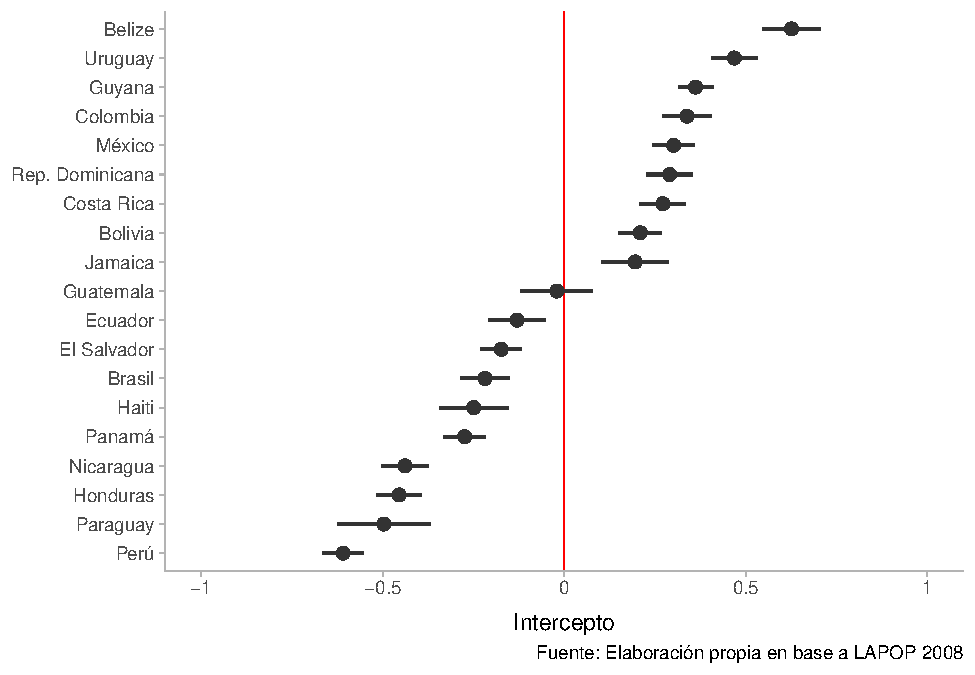
\includegraphics[width=0.8\linewidth]{01-guia_files/figure-latex/fig1-1} 

}

\caption{Interceptos aleatorios por país}\label{fig:fig1}
\end{figure}

\begin{enumerate}
\def\labelenumi{\alph{enumi})}
\setcounter{enumi}{2}
\tightlist
\item
  En base al primer modelo, interprete el efecto de ser casado y de la ideología (5 puntos).
\end{enumerate}

En la Tabla \ref{tab:table1} se muestran los resultados de los modelos multinivel para la confianza política del enunciado 2. Los resultados del Modelo 1 indican que el efecto de estar casado es positivo y estadísticamente significativo (\(\beta\) = 0.05, \(p\) \textless{} 0.01). Específicamente, ceteris paribus, las personas casadas obtienen, en promedio, 0.05 puntos adicionales en la escala de confianza política en comparación con quienes no lo están, siendo este efecto significativo al 99\% de confianza. Por otro lado, el efecto de la ideología política, medida en una escala de 1 a 10 (donde 1 representa posiciones más cercanas a la derecha y 10 a la izquierda), es negativo y estadísticamente significativo con un 99.9\% de confianza. Esto implica que, por cada unidad que aumenta la escala de ideología, la confianza política disminuye en promedio 0.07 puntos, manteniendo constantes los demás predictores.

\begin{enumerate}
\def\labelenumi{\alph{enumi})}
\setcounter{enumi}{3}
\tightlist
\item
  En base al segundo modelo, obtenga las pendientes aleatorias correspondientes al efecto de la ideología y genere manualmente un gráfico que permita visualizar la heterogeneidad de estos efectos. Para ello, mantenga constantes las variables continuas en su media y las variables dicotómicas en la moda muestral. Interprete sustantivamente estos resultados (6 puntos).
\end{enumerate}

La Figura \ref{fig:fig2} presenta las pendientes aleatorias de la ideología política para cada país, junto con una línea punteada que representa la pendiente fija de esta variable en el Modelo 2. A partir de los resultados de este modelo, se observa que, aunque el efecto fijo de la ideología política \emph{entre} países es negativo (\(\beta\) = -0.05, \(p\) \textless{} 0.001), al descomponer este efecto \emph{dentro} de los países se evidencia una heterogeneidad en su dirección. Por ejemplo, en países como El Salvador y Honduras el efecto aleatorio de la ideología es negativo, mientras que en otros, como Uruguay y Haití, es positivo. Estos resultados sugieren que el efecto de la ideología (es decir, ser de izquierda) sobre la confianza política varía entre países; en algunos se asocia con una menor confianza, mientras que en otros con una mayor, lo que releva las diferencias contextuales entre países (que serán objeto de modelamiento en análisis siguientes).

\begin{figure}

{\centering 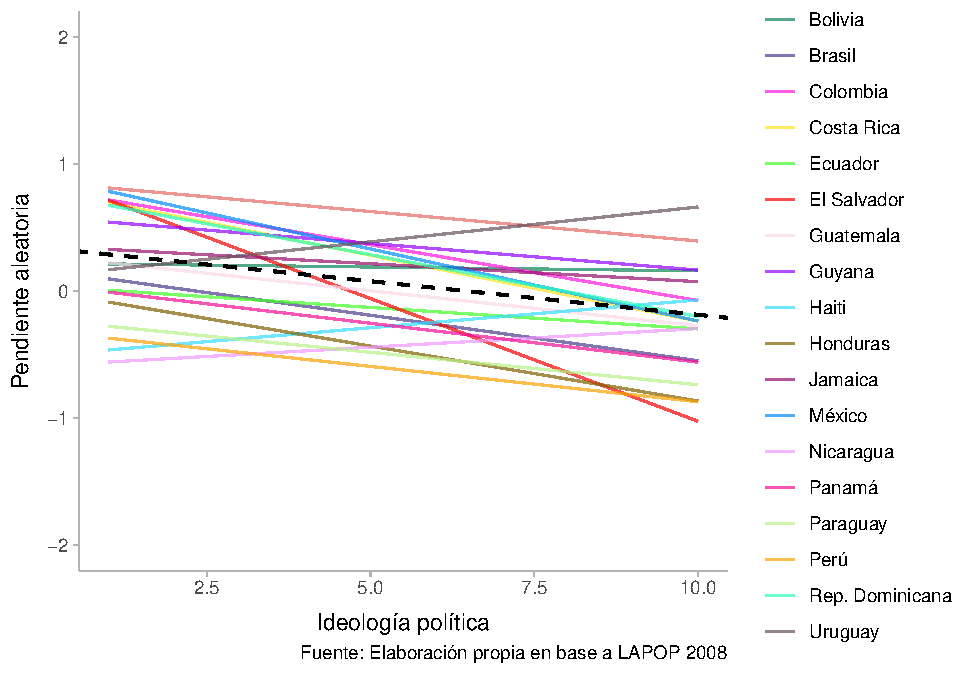
\includegraphics[width=0.8\linewidth]{01-guia_files/figure-latex/fig2-1} 

}

\caption{Pendientes aleatorias de ideología política por país}\label{fig:fig2}
\end{figure}

\begin{enumerate}
\def\labelenumi{\alph{enumi})}
\setcounter{enumi}{4}
\tightlist
\item
  Calcule e intreprete la varianza explicada por el modelo 2. (5 puntos).
\end{enumerate}

Siguiendo a Snijders y Bosker (\protect\hyperlink{ref-snijders_multilevel_2012}{2012}), dado que el Modelo 2 incluye efectos aleatorios de la variable ideología, se utiliza la estimación de la varianza explicada por el Modelo 1 para calcular la varianza explicada por el Modelo 2.

A nivel individual:

\[
R^2_1 = \frac{\sigma^2_{\epsilon}\mid\text{NULO} - \sigma^2_{\epsilon}\mid\text{COMPLETO}}{\sigma^2_{\epsilon}\mid\text{NULO}} = \frac{1.1207 - 1.0932}{1.1207} = 0.025
\]
A nivel contextual:

\[
R^2_2 = \frac{\sigma^2_{\mu_0}\mid\text{NULO} - \sigma^2_{\mu_0}\mid\text{COMPLETO}}{\sigma^2_{\mu_0}\mid\text{NULO}} = \frac{0.1376-0.1369}{0.1376} = 0.005
\]

Los resultados indican que el \(R^2\) a nivel individual \emph{(within)} es de 0.025, mientras que el de nivel contextual \emph{(between)} es de 0.005. De este modo, los predictores individuales del Modelo 1 explican un 2.5\% de la varianza de la confianza política a nivel individual. Por su parte, este modelo solo logra explicar el 0.5\% de la varianza a nivel contextual, lo que corresponde al 0.5\% del 11\% indicado por la correlación intraclase. Con todo, este no es un buen modelo para dar cuenta de la varianza de la confianza política.

\begin{enumerate}
\def\labelenumi{\alph{enumi})}
\setcounter{enumi}{5}
\tightlist
\item
  Tomando como referencia el tercer modelo, obtenga los efectos marginales de ideología moderado por ``presidencia de izquierda''. Interprete sustantivamente estos efectos (6 puntos).
\end{enumerate}

En la Figura \ref{fig:fig3} se muestran los efectos marginales de la ideología moderada por la presencia de presidencia de izquierda en el país, según el Modelo 3. Los resultados indican que, cuando el país cuenta con una presidencia de izquierda (leftpres = 1), el efecto marginal de la ideología es positivo, pero no es estadísticamente significativo al 95\% de confianza (estimación = 0.00243, \(p\) = 0.923). En contraste, cuando el país no tiene una presidencia de izquierda (leftpres = 0), el efecto marginal de la ideología es negativo y estadísticamente significativo (estimación = -0.08163, \(p\) \textless{} 0.001).

\begin{figure}

{\centering 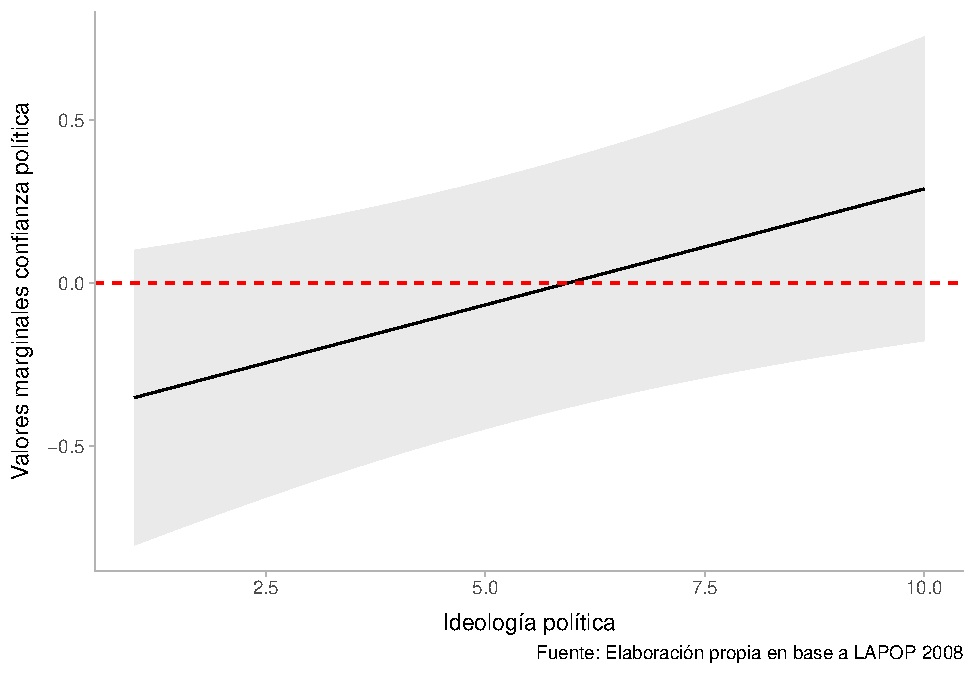
\includegraphics[width=0.8\linewidth]{01-guia_files/figure-latex/fig3-1} 

}

\caption{Efecto marginal de ideología moderado por presidencia de izquierda}\label{fig:fig3}
\end{figure}

Los efectos marginales se pueden expresar con las siguientes ecuaciones:

\begin{enumerate}
\def\labelenumi{\arabic{enumi}.}
\tightlist
\item
  Cuando el país tiene una presidencia de izquierda (leftpres = 1):
\end{enumerate}

\[(\frac{\partial\text{Confianza política}}{\partial\text{Ideología}}\mid\text{Leftpres=1}) = \beta_1\text{Ideología}+\beta_3\text{Ideología x Leftpres}
\]

Donde el efecto marginal estimado de la ideología es 0.00243 con un valor \(p\) de 0.923, el efecto marginal de la ideología es positivo pero no significativo al 95\% de confianza.

\begin{enumerate}
\def\labelenumi{\arabic{enumi}.}
\setcounter{enumi}{1}
\tightlist
\item
  Cuando el país no tiene una presidencia de izquierda (leftpres = 0):
\end{enumerate}

\[(\frac{\partial\text{Confianza política}}{\partial\text{Ideología}}\mid\text{Leftpres=0}) = \beta_1\text{Ideología}
\]

Aquí, el efecto marginal estimado de la ideología es -0.08163 con un valor \(p\) \textless{} 0.001, lo que indica un efecto negativo y estadísticamente significativo.

Con todo, esto sugiere que la influencia de la ideología sobre la confianza política varía dependiendo de la presencia de una presidencia de izquierda, siendo significativa solo en contextos sin dicha presidencia.

\hypertarget{enunciado-3}{%
\section{Enunciado 3}\label{enunciado-3}}

Contraste el modelo 1 estimado en la pregunta 2) con un modelo con la misma estructura fija pero que incorpora efectos aleatorios de la variable edad (modelo 4) y reporte sus resultados en una tabla. Formule la hipótesis apropiada para evaluar si se justifica la inclusión de este parámetro y realice el test estadístico correspondiente. Interprete sus resultados (6 puntos).

En la Tabla \ref{tab:table3} se reportan los estadísticos del análisis de devianza (likelihood ratio test) para el contraste entre el Modelo 1 y 4. La prueba de razón de verosimilitud se utiliza para comparar modelos anidados y determinar cuál se ajusta mejor a los datos (\protect\hyperlink{ref-peugh_practical_2010}{Peugh, 2010}).

La hipótesis nula para esta prueba es que el efecto aleatorio de la edad es igual a cero, mientras que la hipótesis alternativa sostiene que el efecto aleatorio es distinto de cero. Formalmente, las hipótesis son:

\[
H_0 : \sigma^2_{edad} = 0
\]
\[
H_A: \sigma^2_{edad} \neq 0
\]

Los resultados del análisis muestran que la prueba de razón de verosimilitud es estadísticamente significativa, \(\chi^2\) (2) = 75.918, \(p\) \textless{} 0.001. Esto indica que el Modelo 4, que incluye efectos aleatorios para la edad, se ajusta significativamente mejor a los datos que el Modelo 1, que solo considera interceptos aleatorios. Además, el Modelo 4 presenta valores menores de AIC y BIC en comparación con el Modelo 1, lo que refuerza la idea de un mejor ajuste (\protect\hyperlink{ref-hox_multilevel_2017a}{Hox et al., 2017}). Con todo, los resultados sugieren que es posible rechazar la \(H_0\) y entregan evidencia favorable a la \(H_A\) respecto a que el efecto aleatorio de la edad es diferente de cero y mejora el ajuste.

\begin{table}[!h]

\caption{\label{tab:table3}\label{tab:table3} Estadísticos de bondad de ajuste}
\centering
\begin{tabular}[t]{>{\raggedright\arraybackslash}p{2cm}rrrrrl}
\toprule
\textbf{Modelo} & \textbf{AIC} & \textbf{BIC} & \textbf{Deviance} & \textbf{X2} & \textbf{Df} & \textbf{p-value}\\
\midrule
Modelo 1 & 52822.33 & 52900.32 & 52802.33 &  &  & \\
Modelo 4 & 52750.41 & 52844.00 & 52726.41 & 75.92 & 2 & < 0.001 ***\\
\bottomrule
\end{tabular}
\end{table}

\hypertarget{enunciado-4}{%
\section{Enunciado 4}\label{enunciado-4}}

Una de las hipótesis que se trabajan en el artículo de Morgan y Buice (\protect\hyperlink{ref-morgan_latin_2013}{2013}) es que el peso de las mujeres en la fuerza laboral impacta de forma positiva el apoyo a que las mujeres ejerzan roles de liderazgo político. Evalúe esta hipótesis pero utilizando confianza política como variable dependiente. Para ello, estime un modelo en base al modelo 4 pero agregando un efecto fijo de la variable ``Participación femenina en la fuerza laboral'' (FLP). Reporte sus resultados en una tabla. Calcule un test para evaluar la significancia estadística de este efecto y señale a qué nivel de confianza sería estadísticamente significativo (7 puntos).

En la Tabla \ref{tab:table2} se muestran los resultados de los modelos multinivel para la confianza política, incluyendo el Modelo 5, que incorpora un efecto fijo de la participación femenina en la fuerza laboral (FLP). Los resultados del Modelo 5 indican que, aunque el efecto de la participación laboral femenina es positivo (\(\beta = 0.61\)), no es estadísticamente significativo al 95\% de confianza (\(SE = 0.73\), \(p > 0.05\)), manteniendo los demás predictores constantes.

\begin{table}[h!]
\begin{center}
\scalebox{0.9}{
\begin{threeparttable}
\begin{tabular}{l c c c}
\toprule
 & Modelo 4 & Modelo 5 & Modelo 6 \\
\midrule
Intercepto                     & $0.41^{***}$  & $0.08$        & $0.61^{*}$    \\
                               & $(0.08)$      & $(0.41)$      & $(0.24)$      \\
Mujer (Ref.= Hombre)           & $-0.02$       & $-0.02$       & $-0.02$       \\
                               & $(0.02)$      & $(0.02)$      & $(0.02)$      \\
Edad                           & $0.00$        & $0.00$        & $0.09^{*}$    \\
                               & $(0.01)$      & $(0.01)$      & $(0.04)$      \\
Nivel educacional (en años)    & $-0.01^{***}$ & $-0.01^{***}$ & $-0.01^{***}$ \\
                               & $(0.00)$      & $(0.00)$      & $(0.00)$      \\
Empleado (Ref.= Desempleado)   & $-0.05^{*}$   & $-0.05^{*}$   & $-0.04^{*}$   \\
                               & $(0.02)$      & $(0.02)$      & $(0.02)$      \\
Casado (Ref.= Otro)            & $0.05^{**}$   & $0.05^{**}$   & $0.05^{**}$   \\
                               & $(0.02)$      & $(0.02)$      & $(0.02)$      \\
Blanco (Ref.= Otro)            & $-0.02$       & $-0.02$       & $-0.02$       \\
                               & $(0.02)$      & $(0.02)$      & $(0.02)$      \\
Ideología política             & $-0.07^{***}$ & $-0.07^{***}$ & $-0.07^{***}$ \\
                               & $(0.00)$      & $(0.00)$      & $(0.00)$      \\
Participación laboral femenina &               & $0.61$        &               \\
                               &               & $(0.73)$      &               \\
Índice Freedom House           &               &               & $-0.08$       \\
                               &               &               & $(0.09)$      \\
Edad x Índice Freedom House    &               &               & $-0.04^{**}$  \\
                               &               &               & $(0.01)$      \\
\midrule
AIC                            & $52805.69$    & $52805.82$    & $52812.29$    \\
BIC                            & $52899.27$    & $52907.20$    & $52921.47$    \\
Log-likelihood                 & $-26390.84$   & $-26389.91$   & $-26392.14$   \\
Num. obs                       & $18012$       & $18012$       & $18012$       \\
Num. grupos: Países            & $19$          & $19$          & $19$          \\
Var: Países (Intercepto)       & $0.10$        & $0.11$        & $0.10$        \\
Var: Países Edad               & $0.00$        & $0.00$        & $0.00$        \\
Cov: Países (Intercepto), Edad & $0.00$        & $0.00$        & $0.00$        \\
Var: Residual                  & $1.09$        & $1.09$        & $1.09$        \\
\bottomrule
\end{tabular}
\begin{tablenotes}[flushleft]
\scriptsize{\item Nota: Celdas contienen coeficientes de regresión con errores estándares entre paréntesis. $^{***}p<0.001$; $^{**}p<0.01$; $^{*}p<0.05$ \\ \item Fuente: Elaboración propia en base a LAPOP 2008.}
\end{tablenotes}
\end{threeparttable}
}
\caption{\label{tab:table2} Modelos multinivel para confianza política, edad e índice de democracía del país}
\label{table:coefficients}
\end{center}
\end{table}

Para evaluar la significancia estadística de este coeficiente, se realiza un test de Wald. La hipótesis nula (\(H_0\)) es que el coeficiente de la participación laboral femenina es igual a cero:

\[
H_0: \beta_{FLP} = 0
\]

El valor \(z\) se calcula como el cociente entre el coeficiente estimado y su error estándar:

\[
z = \frac{\beta_{FLP}}{SE_{FLP}} = \frac{0.61}{0.73} = 0.83
\]

Este valor \(z\) se compara con el valor crítico de una distribución normal estándar, que es 1.96 para un nivel de significancia \(\alpha = 0.05\). Dado que el valor \(z\) estimado (0.8356) es menor que el valor crítico de 1.96 y el valor \(p\) asociado (0.4163) es mayor que 0.05, no se rechaza la hipótesis nula. Por lo tanto, con un 95\% de confianza, no hay evidencia estadísticamente significativa para apoyar la hipótesis de que la participación laboral femenina tenga un efecto en la confianza política.

Para determinar el nivel de confianza en el que el coeficiente sería estadísticamente significativo, usamos el valor \(z\) = 0.8356, que corresponde a un nivel de significancia (\(\alpha\)) de 0.2027 o 20.27\%. El nivel de confianza vendría siendo 1 - \(\alpha\), lo que resuelve como 1 - 0.2027 = 0.7973. Por tanto, el efecto de la participación laboral femenina sería estadísticamente significativo solo con un nivel de confianza del 79.73\%, lo cual es inferior al nivel de confianza convencial del 95\%.

\hypertarget{enunciado-5}{%
\section{Enunciado 5}\label{enunciado-5}}

En base al modelo 4, especifique un modelo que le permita evaluar si el efecto de la edad es moderado por el Índice de democracia a nivel país (Fredom House Index, fhouse).

\begin{enumerate}
\def\labelenumi{\alph{enumi})}
\tightlist
\item
  Reporte e interprete sustantivamente el intercepto en este modelo (4 puntos)
\end{enumerate}

En la Tabla \ref{tab:table2} se muestran los resultados de los modelos multinivel para la confianza política incorporando el Modelo 6 de este enunciado. De acuerdo con este modelo, el intercepto de este modelo tiene un efecto positivo y estadísticamente significativo (\(\beta\) = 0.61, \(p\) \textless{} 0.05). Este coeficiente representa la confianza política promedio para un individuo típico de referencia, es decir, cuando todas las demás variables predictoras (como sexo, edad, nivel educativo, empleo, casado, raza, ideología, y el índice de democracia) están en sus valores de referencia o cero. En este caso, los valores de referencia serían: hombre, desempleado, no casado, de otra raza (no blanco), con ideología 0, y en un país con el nivel más bajo de democracia (fhouse = 0).

Además, el efecto de interacción entre la edad y el Índice de democracia también afecta la interpretación del intercepto, puesto que, sumado a lo anterior, el impacto de la edad depende del nivel de democracia de los países. Esto significa que, en países con mayores niveles de democracia, el impacto positivo de la edad sobre la confianza política será menor que en países con menores niveles de democracia, debido a la interacción negativa y estadísticamente significativa entre edad y fhouse (\(\beta\) = -0.038, \(p\) \textless{} 0.01).

\begin{figure}

{\centering 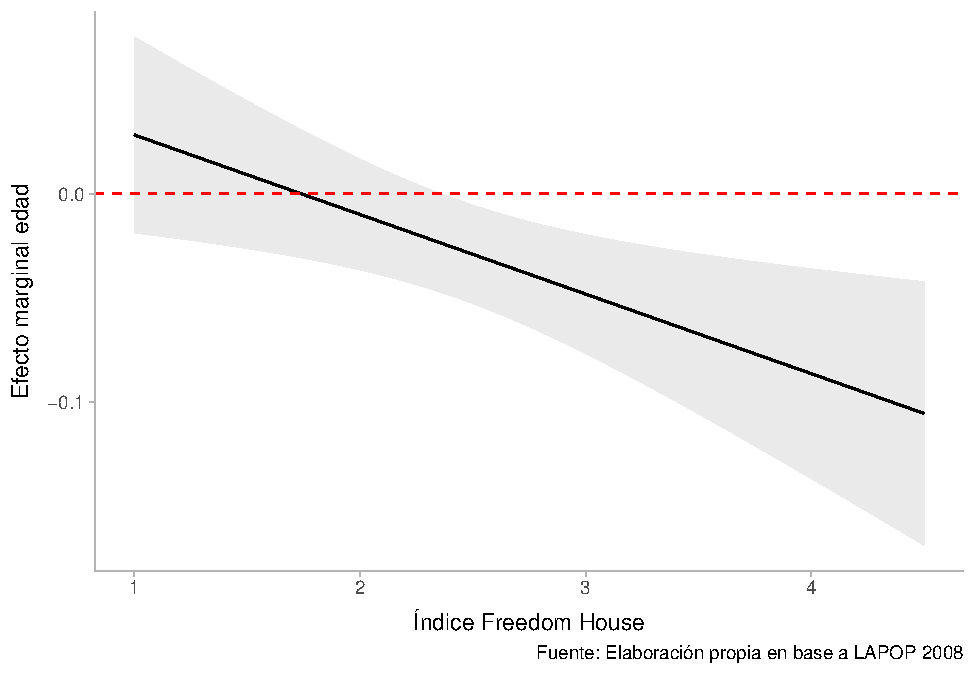
\includegraphics[width=0.8\linewidth]{01-guia_files/figure-latex/fig4-1} 

}

\caption{Efecto marginal de edad moderado por índice de democracia del país}\label{fig:fig4}
\end{figure}

\begin{enumerate}
\def\labelenumi{\alph{enumi})}
\setcounter{enumi}{1}
\tightlist
\item
  Reporte sus resultados a través de un gráfico e interprete sus resultados. ¿Qué se puede concluir en relación al efecto moderador del grado de democracia a nivel país sobre el efecto de la edad? (7 puntos).
\end{enumerate}

En la Figura \ref{fig:fig4} se presentan los efectos marginales de la edad moderados por el nivel de democracia del país, según el Modelo 6. Los resultados sugieren que el efecto marginal de la edad varía significativamente de acuerdo con el nivel del Índice Freedom House (fhouse). En la Tabla \ref{tab:table4} se muestran los efectos marginales estimados para cada valor del Índice Freedom House.

\begin{table}[!h]

\caption{\label{tab:table4}\label{tab:table4} Efectos marginales de edad para valores de Índice Freedom House}
\centering
\begin{tabular}[t]{>{\centering\arraybackslash}p{2cm}cccc}
\toprule
\textbf{Fhouse} & \textbf{Estimación} & \textbf{Error Estándar} & \textbf{Estadístico} & \textbf{p-value}\\
\midrule
1.0 & 0.0282434 & 0.0239885 & 1.1773724 & \\
1.5 & 0.0091603 & 0.0180875 & 0.5064462 & \\
2.0 & -0.0099227 & 0.0135610 & -0.7317095 & \\
2.5 & -0.0290058 & 0.0120586 & -2.4053980 & < 0.05*\\
3.0 & -0.0480889 & 0.0145527 & -3.3044549 & < 0.001***\\
\addlinespace
3.5 & -0.0671719 & 0.0195695 & -3.4324843 & < 0.001***\\
4.5 & -0.1053381 & 0.0322456 & -3.2667441 & < 0.01**\\
\bottomrule
\end{tabular}
\end{table}

De este modo, en países con bajos niveles de democracia (fhouse = 1.0), el efecto de la edad es positivo pero no estadísticamente significativo (\(\beta\) = 0.028, \(p\) = 0.239).Sin embargo, a medida que aumenta el nivel de democracia (fhouse = 2.5 a 4.5), el efecto marginal de la edad se torna negativo y estadísticamente significativo. Por ejemplo, cuando fhouse es 3.0, el efecto es -0.048 (\(p\) \textless{} 0.001) y se vuelve más negativo a medida que el nivel de democracia aumenta, alcanzando -0.105 en fhouse igual a 4.5 (\(p\) \textless{} 0.01).

Esto sugiere que en países con altos niveles de democracia, el impacto de la edad en la confianza política es negativo y más pronunciado, mientras que en países con bajos niveles de democracia, este efecto es insignificante. En definitiva, el grado de democracia modera significativamente el efecto de la edad sobre la confianza política, haciendo que este efecto sea más negativo en contextos más democráticos.

\hypertarget{referencias}{%
\section{Referencias}\label{referencias}}

\hypertarget{refs}{}
\begin{CSLReferences}{1}{0}
\leavevmode\vadjust pre{\hypertarget{ref-finch_multilevel_2014}{}}%
Finch, W. H., Bolin, J. E., \& Kelley, K. (2014). Multilevel {Modeling Using R}.

\leavevmode\vadjust pre{\hypertarget{ref-hox_multilevel_2017a}{}}%
Hox, J., Moerbeek, M., \& Schoot, R. van de. (2017). \emph{Multilevel {Analysis}: {Techniques} and {Applications}, {Third Edition}} (3rd ed.). New York: Routledge. \url{https://doi.org/10.4324/9781315650982}

\leavevmode\vadjust pre{\hypertarget{ref-morgan_latin_2013}{}}%
Morgan, J., \& Buice, M. (2013). Latin {American Attitudes} toward {Women} in {Politics}: {The Influence} of {Elite Cues}, {Female Advancement}, and {Individual Characteristics}. \emph{American Political Science Review}, \emph{107}(4), 644--662. \url{https://doi.org/10.1017/S0003055413000385}

\leavevmode\vadjust pre{\hypertarget{ref-peugh_practical_2010}{}}%
Peugh, J. L. (2010). A practical guide to multilevel modeling. \emph{Journal of School Psychology}, \emph{48}(1), 85--112. \url{https://doi.org/10.1016/j.jsp.2009.09.002}

\leavevmode\vadjust pre{\hypertarget{ref-snijders_multilevel_2012}{}}%
Snijders, T. A. B., \& Bosker, R. J. (2012). \emph{Multilevel analysis: An introduction to basic and advanced multilevel modeling} (2. ed). Los Angeles, Calif.: SAGE.

\end{CSLReferences}

\pagebreak

\hypertarget{cuxf3digo-de-r}{%
\section{Código de R}\label{cuxf3digo-de-r}}

\begin{Shaded}
\begin{Highlighting}[]
\NormalTok{knitr}\SpecialCharTok{::}\NormalTok{opts\_chunk}\SpecialCharTok{$}\FunctionTok{set}\NormalTok{(}\AttributeTok{echo =}\NormalTok{ F,}
                      \AttributeTok{warning =}\NormalTok{ F,}
                      \AttributeTok{error =}\NormalTok{ F, }
                      \AttributeTok{message =}\NormalTok{ F) }
\ControlFlowTok{if}\NormalTok{ (}\SpecialCharTok{!} \FunctionTok{require}\NormalTok{(}\StringTok{"pacman"}\NormalTok{)) }\FunctionTok{install.packages}\NormalTok{(}\StringTok{"pacman"}\NormalTok{)}

\NormalTok{pacman}\SpecialCharTok{::}\FunctionTok{p\_load}\NormalTok{(tidyverse, }
\NormalTok{               sjmisc, }
\NormalTok{               sjPlot, }
\NormalTok{               lme4, }
\NormalTok{               easystats, }
\NormalTok{               influence.ME, }
\NormalTok{               broom.mixed, }
\NormalTok{               here,}
\NormalTok{               texreg, }
\NormalTok{               ggeffects,}
\NormalTok{               marginaleffects,}
\NormalTok{               naniar,}
\NormalTok{               ggdist,}
\NormalTok{               Polychrome,}
\NormalTok{               misty,}
\NormalTok{               kableExtra,}
\NormalTok{               sjlabelled)}

\FunctionTok{options}\NormalTok{(}\AttributeTok{scipen=}\DecValTok{999}\NormalTok{)}
\FunctionTok{rm}\NormalTok{(}\AttributeTok{list =} \FunctionTok{ls}\NormalTok{())}

\NormalTok{miles }\OtherTok{\textless{}{-}} \ControlFlowTok{function}\NormalTok{(x) \{}
  \FunctionTok{format}\NormalTok{(}\FunctionTok{round}\NormalTok{(}\FunctionTok{as.numeric}\NormalTok{(x),}\DecValTok{0}\NormalTok{), }\AttributeTok{big.mark =} \StringTok{"."}\NormalTok{)}
\NormalTok{\}}

\NormalTok{decimales }\OtherTok{\textless{}{-}} \ControlFlowTok{function}\NormalTok{(x) \{}
  \FunctionTok{format}\NormalTok{(}\FunctionTok{round}\NormalTok{(}\FunctionTok{as.numeric}\NormalTok{(x), }\DecValTok{2}\NormalTok{), }\AttributeTok{decimal.mark =} \StringTok{","}\NormalTok{)}
\NormalTok{\}}

\CommentTok{\# set theme}

\FunctionTok{theme\_set}\NormalTok{(}\FunctionTok{theme\_ggdist}\NormalTok{())}

\FunctionTok{options}\NormalTok{(}\AttributeTok{knitr.kable.NA =} \StringTok{""}\NormalTok{)}
\FunctionTok{options}\NormalTok{(}\AttributeTok{knitr.table.format=}\StringTok{"latex"}\NormalTok{)}

\FunctionTok{load}\NormalTok{(}\AttributeTok{file =} \FunctionTok{here}\NormalTok{(}\StringTok{"input/data/morgan2013.RData"}\NormalTok{))}

\FunctionTok{names}\NormalTok{(morgan2013)}
\FunctionTok{glimpse}\NormalTok{(morgan2013)}

\CommentTok{\# seleccionar {-}{-}{-}{-}}

\NormalTok{db }\OtherTok{\textless{}{-}}\NormalTok{ morgan2013 }\SpecialCharTok{\%\textgreater{}\%} 
\NormalTok{  dplyr}\SpecialCharTok{::}\FunctionTok{select}\NormalTok{(country, ID, trustgov, }\AttributeTok{sex =}\NormalTok{ female, age, educ, employed, married, race, }\AttributeTok{ideology =}\NormalTok{ left, leftpres, FLP, fhouse) }\SpecialCharTok{\%\textgreater{}\%} 
\NormalTok{  sjlabelled}\SpecialCharTok{::}\FunctionTok{remove\_all\_labels}\NormalTok{() }\SpecialCharTok{\%\textgreater{}\%} 
\NormalTok{  janitor}\SpecialCharTok{::}\FunctionTok{clean\_names}\NormalTok{() }\SpecialCharTok{\%\textgreater{}\%} 
  \FunctionTok{as\_tibble}\NormalTok{()}
 
\CommentTok{\# filtrar: no {-}{-}{-}{-}{-} }

\CommentTok{\# recodificar y transformar {-}{-}{-}{-}}

\CommentTok{\# trust}
\NormalTok{sjmisc}\SpecialCharTok{::}\FunctionTok{descr}\NormalTok{(db}\SpecialCharTok{$}\NormalTok{in\_trust)}

\CommentTok{\# sexo}
\FunctionTok{frq}\NormalTok{(db}\SpecialCharTok{$}\NormalTok{sex)}

\NormalTok{db}\SpecialCharTok{$}\NormalTok{sex }\OtherTok{\textless{}{-}}\NormalTok{ car}\SpecialCharTok{::}\FunctionTok{recode}\NormalTok{(db}\SpecialCharTok{$}\NormalTok{sex, }
                      \AttributeTok{recodes=} \FunctionTok{c}\NormalTok{(}\StringTok{"0=\textquotesingle{}Hombre\textquotesingle{};1=\textquotesingle{}Mujer\textquotesingle{}"}\NormalTok{),}
                      \AttributeTok{levels =} \FunctionTok{c}\NormalTok{(}\StringTok{"Hombre"}\NormalTok{,}\StringTok{"Mujer"}\NormalTok{),}
                      \AttributeTok{as.factor =}\NormalTok{ T)}

\CommentTok{\# edad}
\NormalTok{sjmisc}\SpecialCharTok{::}\FunctionTok{descr}\NormalTok{(db}\SpecialCharTok{$}\NormalTok{age)}
\FunctionTok{frq}\NormalTok{(db}\SpecialCharTok{$}\NormalTok{age)}

\NormalTok{db}\SpecialCharTok{$}\NormalTok{age\_f }\OtherTok{\textless{}{-}}\NormalTok{ car}\SpecialCharTok{::}\FunctionTok{recode}\NormalTok{(db}\SpecialCharTok{$}\NormalTok{age, }
                      \AttributeTok{recodes =} \FunctionTok{c}\NormalTok{(}\StringTok{"1=\textquotesingle{}Tramo 1\textquotesingle{};}
\StringTok{                                  2=\textquotesingle{}Tramo 2\textquotesingle{};}
\StringTok{                                  3=\textquotesingle{}Tramo 3\textquotesingle{};}
\StringTok{                                  4=\textquotesingle{}Tramo 4\textquotesingle{};}
\StringTok{                                  5=\textquotesingle{}Tramo 5\textquotesingle{};}
\StringTok{                                  6=\textquotesingle{}Tramo 6\textquotesingle{}"}\NormalTok{),}
                      \AttributeTok{levels =} \FunctionTok{c}\NormalTok{(}\StringTok{"Tramo 1"}\NormalTok{,}
                                 \StringTok{"Tramo 2"}\NormalTok{,   }
                                 \StringTok{"Tramo 3"}\NormalTok{,   }
                                 \StringTok{"Tramo 4"}\NormalTok{,    }
                                 \StringTok{"Tramo 5"}\NormalTok{,   }
                                 \StringTok{"Tramo 6"}\NormalTok{),}
                      \AttributeTok{as.factor =}\NormalTok{ T}
\NormalTok{)}

\CommentTok{\# educ}
\NormalTok{sjmisc}\SpecialCharTok{::}\FunctionTok{descr}\NormalTok{(db}\SpecialCharTok{$}\NormalTok{educ)}

\CommentTok{\# employed}
\FunctionTok{frq}\NormalTok{(db}\SpecialCharTok{$}\NormalTok{employed)}

\NormalTok{db}\SpecialCharTok{$}\NormalTok{employed }\OtherTok{\textless{}{-}}\NormalTok{ car}\SpecialCharTok{::}\FunctionTok{recode}\NormalTok{(db}\SpecialCharTok{$}\NormalTok{employed, }
                      \AttributeTok{recodes=} \FunctionTok{c}\NormalTok{(}\StringTok{"0=\textquotesingle{}Desempleado\textquotesingle{};1=\textquotesingle{}Empleado\textquotesingle{}"}\NormalTok{),}
                      \AttributeTok{levels =} \FunctionTok{c}\NormalTok{(}\StringTok{"Desempleado"}\NormalTok{,}\StringTok{"Empleado"}\NormalTok{),}
                      \AttributeTok{as.factor =}\NormalTok{ T)}
\CommentTok{\# married}
\FunctionTok{frq}\NormalTok{(db}\SpecialCharTok{$}\NormalTok{married)}

\NormalTok{db}\SpecialCharTok{$}\NormalTok{married }\OtherTok{\textless{}{-}}\NormalTok{ car}\SpecialCharTok{::}\FunctionTok{recode}\NormalTok{(db}\SpecialCharTok{$}\NormalTok{married, }
                      \AttributeTok{recodes=} \FunctionTok{c}\NormalTok{(}\StringTok{"0=\textquotesingle{}No\textquotesingle{};1=\textquotesingle{}Sí\textquotesingle{}"}\NormalTok{),}
                      \AttributeTok{levels =} \FunctionTok{c}\NormalTok{(}\StringTok{"No"}\NormalTok{,}\StringTok{"Sí"}\NormalTok{),}
                      \AttributeTok{as.factor =}\NormalTok{ T)}

\CommentTok{\# race}
\FunctionTok{frq}\NormalTok{(db}\SpecialCharTok{$}\NormalTok{race)}

\NormalTok{db}\SpecialCharTok{$}\NormalTok{race }\OtherTok{\textless{}{-}}\NormalTok{ car}\SpecialCharTok{::}\FunctionTok{recode}\NormalTok{(db}\SpecialCharTok{$}\NormalTok{race, }
                      \AttributeTok{recodes=} \FunctionTok{c}\NormalTok{(}\StringTok{"0=\textquotesingle{}Otro\textquotesingle{};1=\textquotesingle{}Blanco\textquotesingle{}"}\NormalTok{),}
                      \AttributeTok{levels =} \FunctionTok{c}\NormalTok{(}\StringTok{"Otro"}\NormalTok{,}\StringTok{"Blanco"}\NormalTok{),}
                      \AttributeTok{as.factor =}\NormalTok{ T)}

\CommentTok{\# ideology}
\FunctionTok{frq}\NormalTok{(db}\SpecialCharTok{$}\NormalTok{ideology)}

\CommentTok{\# left}
\FunctionTok{frq}\NormalTok{(db}\SpecialCharTok{$}\NormalTok{leftpres)}

\NormalTok{db}\SpecialCharTok{$}\NormalTok{leftpres }\OtherTok{\textless{}{-}}\NormalTok{ car}\SpecialCharTok{::}\FunctionTok{recode}\NormalTok{(db}\SpecialCharTok{$}\NormalTok{leftpres, }
                      \AttributeTok{recodes=} \FunctionTok{c}\NormalTok{(}\StringTok{"0=\textquotesingle{}No\textquotesingle{};1=\textquotesingle{}Sí\textquotesingle{}"}\NormalTok{),}
                      \AttributeTok{levels =} \FunctionTok{c}\NormalTok{(}\StringTok{"No"}\NormalTok{,}\StringTok{"Sí"}\NormalTok{),}
                      \AttributeTok{as.factor =}\NormalTok{ T)}


\CommentTok{\# flp}
\NormalTok{sjmisc}\SpecialCharTok{::}\FunctionTok{descr}\NormalTok{(db}\SpecialCharTok{$}\NormalTok{flp)}

\CommentTok{\# fhouse}
\NormalTok{sjmisc}\SpecialCharTok{::}\FunctionTok{descr}\NormalTok{(db}\SpecialCharTok{$}\NormalTok{fhouse)}

\CommentTok{\# id}
\NormalTok{sjmisc}\SpecialCharTok{::}\FunctionTok{descr}\NormalTok{(db}\SpecialCharTok{$}\NormalTok{id)}

\CommentTok{\# country}
\FunctionTok{frq}\NormalTok{(db}\SpecialCharTok{$}\NormalTok{country)}

\CommentTok{\# casos perdidos {-}{-}{-}{-}{-}}

\FunctionTok{colSums}\NormalTok{(}\FunctionTok{is.na}\NormalTok{(db))}

\FunctionTok{n\_miss}\NormalTok{(db)}

\FunctionTok{prop\_miss}\NormalTok{(db)}\SpecialCharTok{*}\DecValTok{100}

\FunctionTok{miss\_var\_summary}\NormalTok{(db)}

\FunctionTok{miss\_var\_table}\NormalTok{(db)}

\FunctionTok{vis\_miss}\NormalTok{(db) }\SpecialCharTok{+} \FunctionTok{theme}\NormalTok{(}\AttributeTok{axis.text.x =} \FunctionTok{element\_text}\NormalTok{(}\AttributeTok{angle=}\DecValTok{80}\NormalTok{))}

\NormalTok{db }\OtherTok{\textless{}{-}} \FunctionTok{na.omit}\NormalTok{(db)}

\CommentTok{\# Null model}
\NormalTok{model\_0 }\OtherTok{\textless{}{-}} \FunctionTok{lmer}\NormalTok{(in\_trust }\SpecialCharTok{\textasciitilde{}} \DecValTok{1} \SpecialCharTok{+}\NormalTok{ (}\DecValTok{1} \SpecialCharTok{|}\NormalTok{ country), }
                \AttributeTok{data =}\NormalTok{ db, }\AttributeTok{REML =}\NormalTok{ T)}

\NormalTok{performance}\SpecialCharTok{::}\FunctionTok{icc}\NormalTok{(model\_0, }\AttributeTok{by\_group =}\NormalTok{ T)}
\DocumentationTok{\#\# ICC Country = 0.11}

\NormalTok{sigma\_e }\OtherTok{\textless{}{-}} \FunctionTok{sigma}\NormalTok{(model\_0)}\SpecialCharTok{\^{}}\DecValTok{2}
\NormalTok{tau\_mu }\OtherTok{\textless{}{-}} \FunctionTok{VarCorr}\NormalTok{(model\_0)}\SpecialCharTok{$}\NormalTok{country[[}\DecValTok{1}\NormalTok{]]}
\NormalTok{cic }\OtherTok{\textless{}{-}}\NormalTok{ tau\_mu }\SpecialCharTok{/}\NormalTok{ (tau\_mu}\SpecialCharTok{+}\NormalTok{sigma\_e)}

\CommentTok{\# Influence test}
\NormalTok{inf\_m0 }\OtherTok{\textless{}{-}} \FunctionTok{influence}\NormalTok{(model\_0, }\AttributeTok{group =} \StringTok{"country"}\NormalTok{)}

\CommentTok{\# D cook}
\FunctionTok{cooks.distance}\NormalTok{(inf\_m0, }\AttributeTok{parameters =} \DecValTok{1}\NormalTok{, }\AttributeTok{sort =}\NormalTok{ T) }\CommentTok{\# cut point is 4/19 }

\NormalTok{n\_country }\OtherTok{\textless{}{-}} \FunctionTok{length}\NormalTok{(}\FunctionTok{unique}\NormalTok{(db}\SpecialCharTok{$}\NormalTok{country))}

\FunctionTok{plot}\NormalTok{(inf\_m0, }\AttributeTok{which=}\StringTok{"cook"}\NormalTok{,}
     \AttributeTok{cutoff=}\NormalTok{(}\DecValTok{4}\SpecialCharTok{/}\NormalTok{n\_country), }\AttributeTok{sort=}\ConstantTok{TRUE}\NormalTok{,}
     \AttributeTok{xlab=}\StringTok{"Distancia de Cook"}\NormalTok{,}
     \AttributeTok{ylab=}\StringTok{"País"}\NormalTok{, }\AttributeTok{width=}\DecValTok{60}\NormalTok{, }\AttributeTok{height=}\DecValTok{40}\NormalTok{)}

\CommentTok{\# no obs influyentes}

\CommentTok{\# Modelo 1: Indicadores N1}
\NormalTok{model\_1 }\OtherTok{\textless{}{-}} \FunctionTok{lmer}\NormalTok{(in\_trust }\SpecialCharTok{\textasciitilde{}} \DecValTok{1} \SpecialCharTok{+}\NormalTok{ sex }\SpecialCharTok{+}\NormalTok{ age }\SpecialCharTok{+}\NormalTok{ educ }\SpecialCharTok{+}\NormalTok{ employed }\SpecialCharTok{+}\NormalTok{ married }\SpecialCharTok{+}
\NormalTok{                race }\SpecialCharTok{+}\NormalTok{ ideology }\SpecialCharTok{+}\NormalTok{ (}\DecValTok{1} \SpecialCharTok{|}\NormalTok{ country),}
                \AttributeTok{data =}\NormalTok{ db, }
                \AttributeTok{REML =}\NormalTok{ T)}

\CommentTok{\# Modelo 2: Pendiente aleatoria ideology}
\NormalTok{model\_2 }\OtherTok{\textless{}{-}} \FunctionTok{lmer}\NormalTok{(in\_trust }\SpecialCharTok{\textasciitilde{}} \DecValTok{1} \SpecialCharTok{+}\NormalTok{ sex }\SpecialCharTok{+}\NormalTok{ age }\SpecialCharTok{+}\NormalTok{ educ }\SpecialCharTok{+}\NormalTok{ employed }\SpecialCharTok{+}\NormalTok{ married }\SpecialCharTok{+}
\NormalTok{                race }\SpecialCharTok{+}\NormalTok{ ideology }\SpecialCharTok{+}\NormalTok{ (}\DecValTok{1} \SpecialCharTok{+}\NormalTok{ ideology}\SpecialCharTok{|}\NormalTok{ country),}
                \AttributeTok{data =}\NormalTok{ db, }
                \AttributeTok{REML =}\NormalTok{ T)}

\CommentTok{\# Modelo 3: Interaccion ideology y leftpres}
\NormalTok{model\_3 }\OtherTok{\textless{}{-}} \FunctionTok{lmer}\NormalTok{(in\_trust }\SpecialCharTok{\textasciitilde{}} \DecValTok{1} \SpecialCharTok{+}\NormalTok{ sex }\SpecialCharTok{+}\NormalTok{ age }\SpecialCharTok{+}\NormalTok{ educ }\SpecialCharTok{+}\NormalTok{ employed }\SpecialCharTok{+}\NormalTok{ married }\SpecialCharTok{+}
\NormalTok{                race }\SpecialCharTok{+}\NormalTok{ ideology }\SpecialCharTok{+}\NormalTok{ leftpres }\SpecialCharTok{+}\NormalTok{ ideology}\SpecialCharTok{*}\NormalTok{leftpres }\SpecialCharTok{+} 
\NormalTok{                (}\DecValTok{1} \SpecialCharTok{+}\NormalTok{ ideology}\SpecialCharTok{|}\NormalTok{ country),}
                \AttributeTok{data =}\NormalTok{ db, }
                \AttributeTok{REML =}\NormalTok{ T)}

\CommentTok{\# Modelo 4: Pendiente aleatoria edad}
\NormalTok{model\_4 }\OtherTok{\textless{}{-}} \FunctionTok{lmer}\NormalTok{(in\_trust }\SpecialCharTok{\textasciitilde{}} \DecValTok{1} \SpecialCharTok{+}\NormalTok{ sex }\SpecialCharTok{+}\NormalTok{ age }\SpecialCharTok{+}\NormalTok{ educ }\SpecialCharTok{+}\NormalTok{ employed }\SpecialCharTok{+}\NormalTok{ married }\SpecialCharTok{+}
\NormalTok{                race }\SpecialCharTok{+}\NormalTok{ ideology }\SpecialCharTok{+}\NormalTok{ (}\DecValTok{1} \SpecialCharTok{+}\NormalTok{ age}\SpecialCharTok{|}\NormalTok{ country),}
                \AttributeTok{data =}\NormalTok{ db, }
                \AttributeTok{REML =}\NormalTok{ T)}

\CommentTok{\# Modelo 5: Pendiente aleatoria edad + flp}
\NormalTok{model\_5 }\OtherTok{\textless{}{-}} \FunctionTok{lmer}\NormalTok{(in\_trust }\SpecialCharTok{\textasciitilde{}} \DecValTok{1} \SpecialCharTok{+}\NormalTok{ sex }\SpecialCharTok{+}\NormalTok{ age }\SpecialCharTok{+}\NormalTok{ educ }\SpecialCharTok{+}\NormalTok{ employed }\SpecialCharTok{+}\NormalTok{ married }\SpecialCharTok{+}
\NormalTok{                race }\SpecialCharTok{+}\NormalTok{ ideology }\SpecialCharTok{+}\NormalTok{ flp }\SpecialCharTok{+}\NormalTok{ (}\DecValTok{1} \SpecialCharTok{+}\NormalTok{ age}\SpecialCharTok{|}\NormalTok{ country),}
                \AttributeTok{data =}\NormalTok{ db, }
                \AttributeTok{REML =}\NormalTok{ T)}

\CommentTok{\# Modelo 6: Pendiente aleatoria edad + flp + interaccion fhouse}
\NormalTok{model\_6 }\OtherTok{\textless{}{-}} \FunctionTok{lmer}\NormalTok{(in\_trust }\SpecialCharTok{\textasciitilde{}} \DecValTok{1} \SpecialCharTok{+}\NormalTok{ sex }\SpecialCharTok{+}\NormalTok{ age }\SpecialCharTok{+}\NormalTok{ educ }\SpecialCharTok{+}\NormalTok{ employed }\SpecialCharTok{+}\NormalTok{ married }\SpecialCharTok{+}
\NormalTok{                race }\SpecialCharTok{+}\NormalTok{ ideology }\SpecialCharTok{+}\NormalTok{ age}\SpecialCharTok{*}\NormalTok{fhouse }\SpecialCharTok{+}\NormalTok{ (}\DecValTok{1} \SpecialCharTok{+}\NormalTok{ age}\SpecialCharTok{|}\NormalTok{ country),}
                \AttributeTok{data =}\NormalTok{ db, }
                \AttributeTok{REML =}\NormalTok{ T)}


\NormalTok{ccoef }\OtherTok{\textless{}{-}} \FunctionTok{list}\NormalTok{(}
  \StringTok{"(Intercept)"} \OtherTok{=} \StringTok{"Intercepto"}\NormalTok{,}
  \AttributeTok{sexMujer =} \StringTok{"Mujer (Ref.= Hombre)"}\NormalTok{,}
  \AttributeTok{age =} \StringTok{"Edad"}\NormalTok{,}
  \AttributeTok{educ =} \StringTok{"Nivel educacional (en años)"}\NormalTok{,}
  \AttributeTok{employedEmpleado =} \StringTok{"Empleado (Ref.= Desempleado)"}\NormalTok{,}
\NormalTok{  marriedSí }\OtherTok{=} \StringTok{"Casado (Ref.= Otro)"}\NormalTok{,}
  \AttributeTok{raceBlanco =} \StringTok{"Blanco (Ref.= Otro)"}\NormalTok{,}
  \AttributeTok{ideology =} \StringTok{"Ideología política"}\NormalTok{,}
\NormalTok{  leftpresSí }\OtherTok{=} \StringTok{"Presidencia Izquierda (Ref. = Otra)"}\NormalTok{,}
  \StringTok{"ideology:leftpresSí"} \OtherTok{=} \StringTok{"Ideología política x Presidencia Izquierda (Ref. = Otra)"}\NormalTok{)}


\NormalTok{texreg}\SpecialCharTok{::}\FunctionTok{texreg}\NormalTok{(}\FunctionTok{list}\NormalTok{(model\_1, model\_2, model\_3),}
               \AttributeTok{custom.model.names =} \FunctionTok{c}\NormalTok{(}\StringTok{"Modelo 1"}\NormalTok{,}
                                      \StringTok{"Modelo 2"}\NormalTok{,}
                                      \StringTok{"Modelo 3"}\NormalTok{),}
               \AttributeTok{caption =} \FunctionTok{paste}\NormalTok{(}\StringTok{"(}\SpecialCharTok{\textbackslash{}\textbackslash{}}\StringTok{\#tab:table1)"}\NormalTok{,}\StringTok{"Modelos multinivel para confianza política, ideología política y países con presidencia de izquierda"}\NormalTok{),}
               \AttributeTok{stars =} \FunctionTok{c}\NormalTok{(}\FloatTok{0.05}\NormalTok{, }\FloatTok{0.01}\NormalTok{, }\FloatTok{0.001}\NormalTok{),}
               \AttributeTok{custom.coef.map =}\NormalTok{ ccoef,}
               \AttributeTok{custom.note =} \StringTok{"}\SpecialCharTok{\textbackslash{}\textbackslash{}}\StringTok{item Nota: Celdas contienen coeficientes de regresión con errores estándares entre paréntesis. \%stars }\SpecialCharTok{\textbackslash{}\textbackslash{}\textbackslash{}\textbackslash{}}\StringTok{ }\SpecialCharTok{\textbackslash{}\textbackslash{}}\StringTok{item Fuente: Elaboración propia en base a LAPOP 2008."}\NormalTok{,}
               \AttributeTok{threeparttable =}\NormalTok{ T,}
               \AttributeTok{leading.zero =}\NormalTok{ T,}
               \AttributeTok{float.pos =} \StringTok{"h!"}\NormalTok{,}
               \AttributeTok{use.packages =}\NormalTok{ F,}
               \AttributeTok{booktabs =} \ConstantTok{TRUE}\NormalTok{,}
               \AttributeTok{scalebox =} \FloatTok{0.9}\NormalTok{,}
               \AttributeTok{custom.gof.names =} \FunctionTok{c}\NormalTok{(}\StringTok{"AIC"}\NormalTok{, }
                                    \StringTok{"BIC"}\NormalTok{, }
                                    \StringTok{"Log{-}likelihood"}\NormalTok{, }
                                    \StringTok{"Num. obs"}\NormalTok{, }
                                    \StringTok{"Num. grupos: Países"}\NormalTok{,}
                                    \StringTok{"Var: Países (Intercepto)"}\NormalTok{,}
                                    \StringTok{"Var: Residual"}\NormalTok{,}
                                    \StringTok{"Var: Países Ideología"}\NormalTok{,}
                                    \StringTok{"Cov: Países (Intercepto), Ideología"}
\NormalTok{                                    ))}
\NormalTok{sjPlot}\SpecialCharTok{::}\FunctionTok{plot\_model}\NormalTok{(model\_1, }
                   \AttributeTok{type =} \StringTok{"re"}\NormalTok{, }
                   \AttributeTok{vline.color =} \StringTok{"red"}\NormalTok{,}
                   \AttributeTok{grid =}\NormalTok{ F, }
                   \AttributeTok{sort.est =} \StringTok{"sort.all"}\NormalTok{, }
                   \AttributeTok{ci.lvl =}\NormalTok{ .}\DecValTok{95}\NormalTok{, }
                   \AttributeTok{colors =} \StringTok{"grey20"}\NormalTok{) }\SpecialCharTok{+}
  \FunctionTok{labs}\NormalTok{(}\AttributeTok{title =} \ConstantTok{NULL}\NormalTok{,}
       \AttributeTok{y =} \StringTok{"Intercepto"}\NormalTok{,}
       \AttributeTok{caption =} \StringTok{"Fuente: Elaboración propia en base a LAPOP 2008"}\NormalTok{)}\SpecialCharTok{+}
  \FunctionTok{theme\_ggdist}\NormalTok{()}


\NormalTok{stats\_m2 }\OtherTok{\textless{}{-}}\NormalTok{ broom.mixed}\SpecialCharTok{::}\FunctionTok{tidy}\NormalTok{(model\_2)}

\NormalTok{ideology\_rang }\OtherTok{\textless{}{-}} \FunctionTok{seq}\NormalTok{(}\DecValTok{1}\SpecialCharTok{:}\DecValTok{10}\NormalTok{)}
\NormalTok{in\_trust2 }\OtherTok{\textless{}{-}} \FunctionTok{as.data.frame}\NormalTok{(}\FunctionTok{sapply}\NormalTok{(ideology\_rang,}\ControlFlowTok{function}\NormalTok{(x)}\FunctionTok{fixef}\NormalTok{(model\_2)[}\StringTok{"(Intercept)"}\NormalTok{] }\SpecialCharTok{+} 
                                    \FunctionTok{fixef}\NormalTok{(model\_2)[}\StringTok{"sexMujer"}\NormalTok{]}\SpecialCharTok{*}\DecValTok{0} \SpecialCharTok{+}
                                    \FunctionTok{fixef}\NormalTok{(model\_2)[}\StringTok{"age"}\NormalTok{]}\SpecialCharTok{*}\FloatTok{2.74} \SpecialCharTok{+}
                                    \FunctionTok{fixef}\NormalTok{(model\_2)[}\StringTok{"educ"}\NormalTok{]}\SpecialCharTok{*}\FloatTok{9.23} \SpecialCharTok{+}
                                    \FunctionTok{fixef}\NormalTok{(model\_2)[}\StringTok{"employedEmpleado"}\NormalTok{]}\SpecialCharTok{*}\DecValTok{1} \SpecialCharTok{+}
                                    \FunctionTok{fixef}\NormalTok{(model\_2)[}\StringTok{"marriedSí"}\NormalTok{]}\SpecialCharTok{*}\DecValTok{1} \SpecialCharTok{+}
                                    \FunctionTok{fixef}\NormalTok{(model\_2)[}\StringTok{"raceBlanco"}\NormalTok{]}\SpecialCharTok{*}\DecValTok{0} \SpecialCharTok{+}
                                    \FunctionTok{fixef}\NormalTok{(model\_2)[}\StringTok{"ideology"}\NormalTok{]}\SpecialCharTok{*}\NormalTok{x }\SpecialCharTok{+}
                                    \FunctionTok{ranef}\NormalTok{(model\_2)}\SpecialCharTok{$}\NormalTok{country[,}\DecValTok{1}\NormalTok{] }\SpecialCharTok{+}
                                    \FunctionTok{ranef}\NormalTok{(model\_2)}\SpecialCharTok{$}\NormalTok{country[,}\DecValTok{2}\NormalTok{]}\SpecialCharTok{*}\NormalTok{x))}

\NormalTok{in\_trust2}\SpecialCharTok{$}\NormalTok{country }\OtherTok{\textless{}{-}} \FunctionTok{seq}\NormalTok{(}\DecValTok{1}\SpecialCharTok{:}\DecValTok{19}\NormalTok{)}
\NormalTok{in\_trust2 }\OtherTok{\textless{}{-}} \FunctionTok{reshape}\NormalTok{(in\_trust2,}
                     \AttributeTok{direction =} \StringTok{"long"}\NormalTok{, }\CommentTok{\#formato long}
                     \AttributeTok{v.names =} \StringTok{"pred"}\NormalTok{,}
                     \AttributeTok{varying =} \FunctionTok{list}\NormalTok{(}\FunctionTok{names}\NormalTok{(in\_trust2)[}\DecValTok{1}\SpecialCharTok{:}\DecValTok{10}\NormalTok{]),}
                     \AttributeTok{idvar =} \FunctionTok{c}\NormalTok{(}\StringTok{"country"}\NormalTok{),}
                     \AttributeTok{timevar =} \StringTok{"ideology"}\NormalTok{)}

\NormalTok{colores }\OtherTok{\textless{}{-}} \FunctionTok{setNames}\NormalTok{(}\FunctionTok{createPalette}\NormalTok{(}\DecValTok{19}\NormalTok{, }\FunctionTok{c}\NormalTok{(}\StringTok{"\#E16462"}\NormalTok{, }\StringTok{"\#177b4b"}\NormalTok{, }\StringTok{"\#0D0887"}\NormalTok{)), }\FunctionTok{levels}\NormalTok{(db}\SpecialCharTok{$}\NormalTok{country))}


\NormalTok{in\_trust2 }\SpecialCharTok{\%\textgreater{}\%} 
  \FunctionTok{mutate}\NormalTok{(}\AttributeTok{country =} \FunctionTok{factor}\NormalTok{(country, }
                          \AttributeTok{levels =} \DecValTok{1}\SpecialCharTok{:}\DecValTok{19}\NormalTok{,              }
                          \AttributeTok{labels =} \FunctionTok{levels}\NormalTok{(db}\SpecialCharTok{$}\NormalTok{country))) }\SpecialCharTok{\%\textgreater{}\%} 
  \FunctionTok{ggplot}\NormalTok{(}\FunctionTok{aes}\NormalTok{(}\AttributeTok{x =}\NormalTok{ ideology, }\AttributeTok{y =}\NormalTok{ pred, }\AttributeTok{group =}\NormalTok{ country, }\AttributeTok{color =}\NormalTok{ country)) }\SpecialCharTok{+}
  \FunctionTok{geom\_line}\NormalTok{(}\AttributeTok{alpha =} \FloatTok{0.7}\NormalTok{) }\SpecialCharTok{+} 
  \FunctionTok{ylim}\NormalTok{(}\SpecialCharTok{{-}}\DecValTok{2}\NormalTok{,}\DecValTok{2}\NormalTok{) }\SpecialCharTok{+}
  \FunctionTok{geom\_abline}\NormalTok{(}\AttributeTok{intercept =}\NormalTok{ stats\_m2}\SpecialCharTok{$}\NormalTok{estimate[stats\_m2}\SpecialCharTok{$}\NormalTok{term }\SpecialCharTok{==} \StringTok{"(Intercept)"}\NormalTok{],}
              \AttributeTok{slope =}\NormalTok{ stats\_m2}\SpecialCharTok{$}\NormalTok{estimate[stats\_m2}\SpecialCharTok{$}\NormalTok{term }\SpecialCharTok{==} \StringTok{"ideology"}\NormalTok{],}
              \AttributeTok{color =} \StringTok{"black"}\NormalTok{,}
              \AttributeTok{linetype =} \StringTok{"dashed"}\NormalTok{,}
              \AttributeTok{linewidth =} \FloatTok{0.7}\NormalTok{) }\SpecialCharTok{+}
  \FunctionTok{scale\_color\_manual}\NormalTok{(}\AttributeTok{values =}\NormalTok{ colores) }\SpecialCharTok{+}
  \FunctionTok{labs}\NormalTok{(}\AttributeTok{y =} \StringTok{"Pendiente aleatoria"}\NormalTok{,}
       \AttributeTok{x =} \StringTok{"Ideología política"}\NormalTok{,}
       \AttributeTok{color =} \StringTok{"País"}\NormalTok{,}
       \AttributeTok{caption =} \StringTok{"Fuente: Elaboración propia en base a LAPOP 2008"}\NormalTok{) }


\CommentTok{\# manual}

\NormalTok{varcomp\_0 }\OtherTok{\textless{}{-}} \FunctionTok{as.data.frame}\NormalTok{(}\FunctionTok{VarCorr}\NormalTok{(model\_0))}
\NormalTok{tau00\_0 }\OtherTok{\textless{}{-}}\NormalTok{ varcomp\_0[}\DecValTok{1}\NormalTok{,}\DecValTok{4}\NormalTok{]}
\NormalTok{sigma2\_0 }\OtherTok{\textless{}{-}}\NormalTok{ varcomp\_0[}\DecValTok{2}\NormalTok{,}\DecValTok{4}\NormalTok{]}

\NormalTok{varcomp\_1 }\OtherTok{\textless{}{-}} \FunctionTok{as.data.frame}\NormalTok{(}\FunctionTok{VarCorr}\NormalTok{(model\_1))}
\NormalTok{tau00\_1 }\OtherTok{\textless{}{-}}\NormalTok{ varcomp\_1[}\DecValTok{1}\NormalTok{,}\DecValTok{4}\NormalTok{]}
\NormalTok{sigma2\_1 }\OtherTok{\textless{}{-}}\NormalTok{ varcomp\_1[}\DecValTok{2}\NormalTok{,}\DecValTok{4}\NormalTok{]}

\NormalTok{R2\_1\_L1 }\OtherTok{\textless{}{-}}\NormalTok{ (sigma2\_0}\SpecialCharTok{{-}}\NormalTok{sigma2\_1)}\SpecialCharTok{/}\NormalTok{sigma2\_0}
\NormalTok{R2\_1\_L1}

\NormalTok{R2\_2\_L1 }\OtherTok{\textless{}{-}}\NormalTok{ (tau00\_0}\SpecialCharTok{{-}}\NormalTok{tau00\_1)}\SpecialCharTok{/}\NormalTok{tau00\_0}
\NormalTok{R2\_2\_L1}

\CommentTok{\# misty}
\NormalTok{db\_n }\OtherTok{\textless{}{-}}\NormalTok{ db }\SpecialCharTok{\%\textgreater{}\%} 
  \FunctionTok{mutate}\NormalTok{(}
    \FunctionTok{across}\NormalTok{(}\AttributeTok{.cols =} \FunctionTok{c}\NormalTok{(sex, age, employed, married, race),}
           \AttributeTok{.fns =} \SpecialCharTok{\textasciitilde{}} \FunctionTok{as.numeric}\NormalTok{(.))}
\NormalTok{  )}
 

\NormalTok{model\_1\_n }\OtherTok{\textless{}{-}} \FunctionTok{lmer}\NormalTok{(in\_trust }\SpecialCharTok{\textasciitilde{}} \DecValTok{1} \SpecialCharTok{+}\NormalTok{ sex }\SpecialCharTok{+}\NormalTok{ age }\SpecialCharTok{+}\NormalTok{ educ }\SpecialCharTok{+}\NormalTok{ employed }\SpecialCharTok{+}\NormalTok{ married }\SpecialCharTok{+}
\NormalTok{                race }\SpecialCharTok{+}\NormalTok{ ideology }\SpecialCharTok{+}\NormalTok{ (}\DecValTok{1} \SpecialCharTok{|}\NormalTok{ country),}
                \AttributeTok{data =}\NormalTok{ db\_n, }
                \AttributeTok{REML =}\NormalTok{ T)}

\NormalTok{misty}\SpecialCharTok{::}\FunctionTok{multilevel.r2}\NormalTok{(}\AttributeTok{model =}\NormalTok{ model\_1\_n, }\AttributeTok{print =} \StringTok{"all"}\NormalTok{)}


\FunctionTok{plot\_slopes}\NormalTok{(model\_3, }
            \AttributeTok{variables =} \StringTok{"ideology"}\NormalTok{, }
            \AttributeTok{condition =} \StringTok{"leftpres"}\NormalTok{,}
            \AttributeTok{conf\_level =}\NormalTok{ .}\DecValTok{95}\NormalTok{) }\SpecialCharTok{+}
  \FunctionTok{geom\_hline}\NormalTok{(}\AttributeTok{yintercept =} \DecValTok{0}\NormalTok{, }
             \AttributeTok{color =} \StringTok{"red"}\NormalTok{, }
             \AttributeTok{linetype =} \StringTok{"dashed"}\NormalTok{) }\SpecialCharTok{+}
  \FunctionTok{labs}\NormalTok{(}\AttributeTok{y =} \StringTok{"Efecto marginal ideología política"}\NormalTok{,}
       \AttributeTok{x =} \StringTok{"Presidencia de izquierda"}\NormalTok{,}
       \AttributeTok{caption =} \StringTok{"Fuente: Elaboración propia en base a LAPOP 2008"}\NormalTok{,}
       \AttributeTok{title =} \ConstantTok{NULL}\NormalTok{)}


\CommentTok{\#performance::test\_likelihoodratio(model\_1, model\_4)}

\NormalTok{res\_fit1 }\OtherTok{\textless{}{-}} \FunctionTok{anova}\NormalTok{(model\_1, model\_4)}

\NormalTok{fit\_tab }\OtherTok{\textless{}{-}}\NormalTok{ res\_fit1[}\FunctionTok{c}\NormalTok{(}\DecValTok{2}\NormalTok{,}\DecValTok{3}\NormalTok{,}\DecValTok{5}\NormalTok{,}\DecValTok{6}\NormalTok{,}\DecValTok{7}\NormalTok{,}\DecValTok{8}\NormalTok{)] }\SpecialCharTok{\%\textgreater{}\%} \FunctionTok{as.tibble}\NormalTok{(.)}

\NormalTok{fit\_tab}\SpecialCharTok{$}\NormalTok{mod }\OtherTok{\textless{}{-}} \FunctionTok{c}\NormalTok{(}\StringTok{"Modelo 1"}\NormalTok{, }\StringTok{"Modelo 4"}\NormalTok{)}

\NormalTok{fit\_tab}\SpecialCharTok{$}\NormalTok{p }\OtherTok{\textless{}{-}} \FunctionTok{if\_else}\NormalTok{(fit\_tab}\SpecialCharTok{$}\StringTok{\textasciigrave{}}\AttributeTok{Pr(\textgreater{}Chisq)}\StringTok{\textasciigrave{}} \SpecialCharTok{\textless{}} \FloatTok{0.001}\NormalTok{, }\StringTok{"\textless{} 0.001 ***"}\NormalTok{, }\ConstantTok{NA}\NormalTok{)}

\NormalTok{fit\_tab}\SpecialCharTok{$}\NormalTok{Chisq }\OtherTok{\textless{}{-}} \FunctionTok{round}\NormalTok{(fit\_tab}\SpecialCharTok{$}\NormalTok{Chisq, }\AttributeTok{digits =} \DecValTok{2}\NormalTok{)}

\NormalTok{fit\_tab }\OtherTok{\textless{}{-}}\NormalTok{ fit\_tab }\SpecialCharTok{\%\textgreater{}\%} 
  \FunctionTok{select}\NormalTok{(mod, AIC, BIC, deviance, Chisq, Df, p)}

\NormalTok{colnames }\OtherTok{\textless{}{-}} \FunctionTok{c}\NormalTok{(}\StringTok{"Modelo"}\NormalTok{, }\StringTok{"AIC"}\NormalTok{, }\StringTok{"BIC"}\NormalTok{, }\StringTok{"Deviance"}\NormalTok{, }\StringTok{"X2"}\NormalTok{, }\StringTok{"Df"}\NormalTok{, }\StringTok{"p{-}value"}\NormalTok{)}

\NormalTok{fit\_tab }\OtherTok{\textless{}{-}}\NormalTok{ kableExtra}\SpecialCharTok{::}\FunctionTok{kable}\NormalTok{(fit\_tab, }
                             \AttributeTok{format =} \StringTok{"latex"}\NormalTok{, }
                             \AttributeTok{col.names =}\NormalTok{ colnames,}
                             \AttributeTok{row.names =}\NormalTok{ F,}
                             \AttributeTok{booktabs =}\NormalTok{ T, }
                             \AttributeTok{caption =} \FunctionTok{paste}\NormalTok{(}\StringTok{"(}\SpecialCharTok{\textbackslash{}\textbackslash{}}\StringTok{\#tab:table3)"}\NormalTok{,}\StringTok{"Estadísticos de bondad de ajuste"}\NormalTok{),) }\SpecialCharTok{\%\textgreater{}\%} 
\NormalTok{  kableExtra}\SpecialCharTok{::}\FunctionTok{kable\_styling}\NormalTok{(}\AttributeTok{latex\_options =} \StringTok{"hold\_position"}\NormalTok{, }
                            \AttributeTok{position =} \StringTok{"center"}\NormalTok{) }\SpecialCharTok{\%\textgreater{}\%}
\NormalTok{  kableExtra}\SpecialCharTok{::}\FunctionTok{kable\_styling}\NormalTok{(}\AttributeTok{bootstrap\_options =} \FunctionTok{c}\NormalTok{(}\StringTok{"striped"}\NormalTok{, }\StringTok{"hover"}\NormalTok{, }\StringTok{"condensed"}\NormalTok{, }\StringTok{"responsive"}\NormalTok{), }\AttributeTok{full\_width =}\NormalTok{ F) }\SpecialCharTok{\%\textgreater{}\%} 
  \FunctionTok{column\_spec}\NormalTok{(}\DecValTok{1}\NormalTok{, }\AttributeTok{width =} \StringTok{"2cm"}\NormalTok{) }\SpecialCharTok{\%\textgreater{}\%}
  \FunctionTok{row\_spec}\NormalTok{(}\DecValTok{0}\NormalTok{, }\AttributeTok{bold =}\NormalTok{ T)}

\NormalTok{fit\_tab}


\NormalTok{ccoef }\OtherTok{\textless{}{-}} \FunctionTok{list}\NormalTok{(}
  \StringTok{"(Intercept)"} \OtherTok{=} \StringTok{"Intercepto"}\NormalTok{,}
  \AttributeTok{sexMujer =} \StringTok{"Mujer (Ref.= Hombre)"}\NormalTok{,}
  \AttributeTok{age =} \StringTok{"Edad"}\NormalTok{,}
  \AttributeTok{educ =} \StringTok{"Nivel educacional (en años)"}\NormalTok{,}
  \AttributeTok{employedEmpleado =} \StringTok{"Empleado (Ref.= Desempleado)"}\NormalTok{,}
\NormalTok{  marriedSí }\OtherTok{=} \StringTok{"Casado (Ref.= Otro)"}\NormalTok{,}
  \AttributeTok{raceBlanco =} \StringTok{"Blanco (Ref.= Otro)"}\NormalTok{,}
  \AttributeTok{ideology =} \StringTok{"Ideología política"}\NormalTok{,}
  \AttributeTok{flp =} \StringTok{"Participación laboral femenina"}\NormalTok{,}
  \AttributeTok{fhouse =} \StringTok{"Índice Freedom House"}\NormalTok{,}
  \StringTok{"age:fhouse"} \OtherTok{=} \StringTok{"Edad x Índice Freedom House"}
\NormalTok{)}


\NormalTok{texreg}\SpecialCharTok{::}\FunctionTok{texreg}\NormalTok{(}\FunctionTok{list}\NormalTok{(model\_4, model\_5, model\_6),}
               \AttributeTok{custom.model.names =} \FunctionTok{c}\NormalTok{(}\StringTok{"Modelo 4"}\NormalTok{,}
                                      \StringTok{"Modelo 5"}\NormalTok{,}
                                      \StringTok{"Modelo 6"}\NormalTok{),}
               \AttributeTok{caption =} \FunctionTok{paste}\NormalTok{(}\StringTok{"(}\SpecialCharTok{\textbackslash{}\textbackslash{}}\StringTok{\#tab:table2)"}\NormalTok{,}\StringTok{"Modelos multinivel para confianza política, edad e índice de democracía del país"}\NormalTok{),}
               \AttributeTok{stars =} \FunctionTok{c}\NormalTok{(}\FloatTok{0.05}\NormalTok{, }\FloatTok{0.01}\NormalTok{, }\FloatTok{0.001}\NormalTok{),}
               \AttributeTok{custom.coef.map =}\NormalTok{ ccoef,}
               \AttributeTok{custom.note =} \StringTok{"}\SpecialCharTok{\textbackslash{}\textbackslash{}}\StringTok{item Nota: Celdas contienen coeficientes de regresión con errores estándares entre paréntesis. \%stars }\SpecialCharTok{\textbackslash{}\textbackslash{}\textbackslash{}\textbackslash{}}\StringTok{ }\SpecialCharTok{\textbackslash{}\textbackslash{}}\StringTok{item Fuente: Elaboración propia en base a LAPOP 2008."}\NormalTok{,}
               \AttributeTok{threeparttable =}\NormalTok{ T,}
               \AttributeTok{leading.zero =}\NormalTok{ T,}
               \AttributeTok{float.pos =} \StringTok{"h!"}\NormalTok{,}
               \AttributeTok{use.packages =}\NormalTok{ F,}
               \AttributeTok{booktabs =} \ConstantTok{TRUE}\NormalTok{,}
               \AttributeTok{scalebox =} \FloatTok{0.9}\NormalTok{,}
               \AttributeTok{custom.gof.names =} \FunctionTok{c}\NormalTok{(}\StringTok{"AIC"}\NormalTok{, }
                                    \StringTok{"BIC"}\NormalTok{, }
                                    \StringTok{"Log{-}likelihood"}\NormalTok{, }
                                    \StringTok{"Num. obs"}\NormalTok{, }
                                    \StringTok{"Num. grupos: Países"}\NormalTok{,}
                                    \StringTok{"Var: Países (Intercepto)"}\NormalTok{,}
                                    \StringTok{"Var: Países Edad"}\NormalTok{,}
                                    \StringTok{"Cov: Países (Intercepto), Edad"}\NormalTok{,}
                                    \StringTok{"Var: Residual"}
                                     
\NormalTok{                                    ))}

\NormalTok{n2 }\OtherTok{\textless{}{-}} \FunctionTok{length}\NormalTok{(}\FunctionTok{unique}\NormalTok{(db}\SpecialCharTok{$}\NormalTok{country))}

\NormalTok{z\_fpl }\OtherTok{\textless{}{-}}\NormalTok{ (}\FunctionTok{fixef}\NormalTok{(model\_5)[}\DecValTok{9}\NormalTok{])}\SpecialCharTok{/}\NormalTok{(}\FunctionTok{sqrt}\NormalTok{(}\FunctionTok{diag}\NormalTok{(}\FunctionTok{vcov}\NormalTok{(model\_5))[}\DecValTok{9}\NormalTok{]))}

\NormalTok{pval\_flp }\OtherTok{\textless{}{-}} \DecValTok{2} \SpecialCharTok{*} \FunctionTok{pt}\NormalTok{(}\SpecialCharTok{{-}}\FunctionTok{abs}\NormalTok{(z\_fpl), }\AttributeTok{df=}\NormalTok{n2}\DecValTok{{-}1{-}1}\NormalTok{, }\AttributeTok{lower.tail =}\NormalTok{ T)}

\FunctionTok{model\_parameters}\NormalTok{(model\_5, }\AttributeTok{ci\_method =} \StringTok{"wald"}\NormalTok{, }\AttributeTok{summary =}\NormalTok{ T)}


\FunctionTok{plot\_slopes}\NormalTok{(model\_6, }
            \AttributeTok{variables =} \StringTok{"age"}\NormalTok{, }
            \AttributeTok{condition =} \StringTok{"fhouse"}\NormalTok{,}
            \AttributeTok{conf\_level =}\NormalTok{ .}\DecValTok{95}\NormalTok{) }\SpecialCharTok{+}
  \FunctionTok{geom\_hline}\NormalTok{(}\AttributeTok{yintercept =} \FloatTok{0.0}\NormalTok{, }
             \AttributeTok{color =} \StringTok{"red"}\NormalTok{, }
             \AttributeTok{linetype =} \StringTok{"dashed"}\NormalTok{) }\SpecialCharTok{+}
  \FunctionTok{labs}\NormalTok{(}\AttributeTok{y =} \StringTok{"Efecto marginal edad"}\NormalTok{,}
       \AttributeTok{x =} \StringTok{"Índice Freedom House"}\NormalTok{,}
       \AttributeTok{caption =} \StringTok{"Fuente: Elaboración propia en base a LAPOP 2008"}\NormalTok{,}
       \AttributeTok{title =} \ConstantTok{NULL}\NormalTok{)}


\FunctionTok{slopes}\NormalTok{(model\_6, }\AttributeTok{variables =} \StringTok{"age"}\NormalTok{, }\AttributeTok{by =} \StringTok{"fhouse"}\NormalTok{, }\AttributeTok{newdata =} \StringTok{"mean"}\NormalTok{) }\SpecialCharTok{\%\textgreater{}\%} 
  \FunctionTok{tidy}\NormalTok{() }\SpecialCharTok{\%\textgreater{}\%} 
  \FunctionTok{select}\NormalTok{(}\DecValTok{4}\SpecialCharTok{:}\DecValTok{8}\NormalTok{) }\SpecialCharTok{\%\textgreater{}\%} 
  \FunctionTok{mutate}\NormalTok{(}\AttributeTok{p =} \FunctionTok{case\_when}\NormalTok{(p.value }\SpecialCharTok{\textless{}} \FloatTok{0.05} \SpecialCharTok{\&}\NormalTok{ p.value }\SpecialCharTok{\textgreater{}} \FloatTok{0.01} \SpecialCharTok{\textasciitilde{}} \StringTok{"\textless{} 0.05*"}\NormalTok{,}
\NormalTok{                       p.value }\SpecialCharTok{\textless{}} \FloatTok{0.01} \SpecialCharTok{\&}\NormalTok{ p.value }\SpecialCharTok{\textgreater{}} \FloatTok{0.001} \SpecialCharTok{\textasciitilde{}} \StringTok{"\textless{} 0.01**"}\NormalTok{,}
\NormalTok{                       p.value }\SpecialCharTok{\textless{}} \FloatTok{0.001} \SpecialCharTok{\textasciitilde{}} \StringTok{"\textless{} 0.001***"}\NormalTok{,}
                       \ConstantTok{TRUE} \SpecialCharTok{\textasciitilde{}} \StringTok{""}\NormalTok{)) }\SpecialCharTok{\%\textgreater{}\%} 
  \FunctionTok{select}\NormalTok{(}\SpecialCharTok{{-}}\NormalTok{p.value) }\SpecialCharTok{\%\textgreater{}\%} 
\NormalTok{  kableExtra}\SpecialCharTok{::}\FunctionTok{kable}\NormalTok{(}\AttributeTok{format =} \StringTok{"latex"}\NormalTok{, }
                    \AttributeTok{col.names =} \FunctionTok{c}\NormalTok{(}\StringTok{"Fhouse"}\NormalTok{, }\StringTok{"Estimación"}\NormalTok{, }\StringTok{"Error Estándar"}\NormalTok{, }\StringTok{"Estadístico"}\NormalTok{, }\StringTok{"p{-}value"}\NormalTok{),}
                    \AttributeTok{row.names =}\NormalTok{ F,}
                    \AttributeTok{booktabs =}\NormalTok{ T, }\AttributeTok{align =} \StringTok{\textquotesingle{}c\textquotesingle{}}\NormalTok{,}
                    \AttributeTok{caption =} \FunctionTok{paste}\NormalTok{(}\StringTok{"(}\SpecialCharTok{\textbackslash{}\textbackslash{}}\StringTok{\#tab:table4)"}\NormalTok{,}\StringTok{"Efectos marginales de edad para valores de Índice Freedom House"}\NormalTok{)) }\SpecialCharTok{\%\textgreater{}\%} 
\NormalTok{  kableExtra}\SpecialCharTok{::}\FunctionTok{kable\_styling}\NormalTok{(}\AttributeTok{latex\_options =} \StringTok{"hold\_position"}\NormalTok{, }
                            \AttributeTok{position =} \StringTok{"center"}\NormalTok{) }\SpecialCharTok{\%\textgreater{}\%}
\NormalTok{  kableExtra}\SpecialCharTok{::}\FunctionTok{kable\_styling}\NormalTok{(}\AttributeTok{bootstrap\_options =} \FunctionTok{c}\NormalTok{(}\StringTok{"striped"}\NormalTok{, }\StringTok{"hover"}\NormalTok{, }\StringTok{"condensed"}\NormalTok{, }\StringTok{"responsive"}\NormalTok{), }\AttributeTok{full\_width =}\NormalTok{ F) }\SpecialCharTok{\%\textgreater{}\%} 
  \FunctionTok{column\_spec}\NormalTok{(}\DecValTok{1}\NormalTok{, }\AttributeTok{width =} \StringTok{"2cm"}\NormalTok{) }\SpecialCharTok{\%\textgreater{}\%}
  \FunctionTok{row\_spec}\NormalTok{(}\DecValTok{0}\NormalTok{, }\AttributeTok{bold =}\NormalTok{ T)}
\end{Highlighting}
\end{Shaded}


\end{document}
